% Options for packages loaded elsewhere
\PassOptionsToPackage{unicode}{hyperref}
\PassOptionsToPackage{hyphens}{url}
%
\documentclass[
  ignorenonframetext,
]{beamer}
\usepackage{pgfpages}
\setbeamertemplate{caption}[numbered]
\setbeamertemplate{caption label separator}{: }
\setbeamercolor{caption name}{fg=normal text.fg}
\beamertemplatenavigationsymbolsempty
% Prevent slide breaks in the middle of a paragraph
\widowpenalties 1 10000
\raggedbottom
\setbeamertemplate{part page}{
  \centering
  \begin{beamercolorbox}[sep=16pt,center]{part title}
    \usebeamerfont{part title}\insertpart\par
  \end{beamercolorbox}
}
\setbeamertemplate{section page}{
  \centering
  \begin{beamercolorbox}[sep=12pt,center]{part title}
    \usebeamerfont{section title}\insertsection\par
  \end{beamercolorbox}
}
\setbeamertemplate{subsection page}{
  \centering
  \begin{beamercolorbox}[sep=8pt,center]{part title}
    \usebeamerfont{subsection title}\insertsubsection\par
  \end{beamercolorbox}
}
\AtBeginPart{
  \frame{\partpage}
}
\AtBeginSection{
  \ifbibliography
  \else
    \frame{\sectionpage}
  \fi
}
\AtBeginSubsection{
  \frame{\subsectionpage}
}

\usepackage{amsmath,amssymb}
\usepackage{iftex}
\ifPDFTeX
  \usepackage[T1]{fontenc}
  \usepackage[utf8]{inputenc}
  \usepackage{textcomp} % provide euro and other symbols
\else % if luatex or xetex
  \usepackage{unicode-math}
  \defaultfontfeatures{Scale=MatchLowercase}
  \defaultfontfeatures[\rmfamily]{Ligatures=TeX,Scale=1}
\fi
\usepackage{lmodern}
\ifPDFTeX\else  
    % xetex/luatex font selection
\fi
% Use upquote if available, for straight quotes in verbatim environments
\IfFileExists{upquote.sty}{\usepackage{upquote}}{}
\IfFileExists{microtype.sty}{% use microtype if available
  \usepackage[]{microtype}
  \UseMicrotypeSet[protrusion]{basicmath} % disable protrusion for tt fonts
}{}
\makeatletter
\@ifundefined{KOMAClassName}{% if non-KOMA class
  \IfFileExists{parskip.sty}{%
    \usepackage{parskip}
  }{% else
    \setlength{\parindent}{0pt}
    \setlength{\parskip}{6pt plus 2pt minus 1pt}}
}{% if KOMA class
  \KOMAoptions{parskip=half}}
\makeatother
\usepackage{xcolor}
\newif\ifbibliography
\setlength{\emergencystretch}{3em} % prevent overfull lines
\setcounter{secnumdepth}{-\maxdimen} % remove section numbering


\providecommand{\tightlist}{%
  \setlength{\itemsep}{0pt}\setlength{\parskip}{0pt}}\usepackage{longtable,booktabs,array}
\usepackage{calc} % for calculating minipage widths
\usepackage{caption}
% Make caption package work with longtable
\makeatletter
\def\fnum@table{\tablename~\thetable}
\makeatother
\usepackage{graphicx}
\makeatletter
\def\maxwidth{\ifdim\Gin@nat@width>\linewidth\linewidth\else\Gin@nat@width\fi}
\def\maxheight{\ifdim\Gin@nat@height>\textheight\textheight\else\Gin@nat@height\fi}
\makeatother
% Scale images if necessary, so that they will not overflow the page
% margins by default, and it is still possible to overwrite the defaults
% using explicit options in \includegraphics[width, height, ...]{}
\setkeys{Gin}{width=\maxwidth,height=\maxheight,keepaspectratio}
% Set default figure placement to htbp
\makeatletter
\def\fps@figure{htbp}
\makeatother
% definitions for citeproc citations
\NewDocumentCommand\citeproctext{}{}
\NewDocumentCommand\citeproc{mm}{%
  \begingroup\def\citeproctext{#2}\cite{#1}\endgroup}
\makeatletter
 % allow citations to break across lines
 \let\@cite@ofmt\@firstofone
 % avoid brackets around text for \cite:
 \def\@biblabel#1{}
 \def\@cite#1#2{{#1\if@tempswa , #2\fi}}
\makeatother
\newlength{\cslhangindent}
\setlength{\cslhangindent}{1.5em}
\newlength{\csllabelwidth}
\setlength{\csllabelwidth}{3em}
\newenvironment{CSLReferences}[2] % #1 hanging-indent, #2 entry-spacing
 {\begin{list}{}{%
  \setlength{\itemindent}{0pt}
  \setlength{\leftmargin}{0pt}
  \setlength{\parsep}{0pt}
  % turn on hanging indent if param 1 is 1
  \ifodd #1
   \setlength{\leftmargin}{\cslhangindent}
   \setlength{\itemindent}{-1\cslhangindent}
  \fi
  % set entry spacing
  \setlength{\itemsep}{#2\baselineskip}}}
 {\end{list}}
\usepackage{calc}
\newcommand{\CSLBlock}[1]{\hfill\break\parbox[t]{\linewidth}{\strut\ignorespaces#1\strut}}
\newcommand{\CSLLeftMargin}[1]{\parbox[t]{\csllabelwidth}{\strut#1\strut}}
\newcommand{\CSLRightInline}[1]{\parbox[t]{\linewidth - \csllabelwidth}{\strut#1\strut}}
\newcommand{\CSLIndent}[1]{\hspace{\cslhangindent}#1}

\makeatletter
\@ifpackageloaded{caption}{}{\usepackage{caption}}
\AtBeginDocument{%
\ifdefined\contentsname
  \renewcommand*\contentsname{Table of contents}
\else
  \newcommand\contentsname{Table of contents}
\fi
\ifdefined\listfigurename
  \renewcommand*\listfigurename{List of Figures}
\else
  \newcommand\listfigurename{List of Figures}
\fi
\ifdefined\listtablename
  \renewcommand*\listtablename{List of Tables}
\else
  \newcommand\listtablename{List of Tables}
\fi
\ifdefined\figurename
  \renewcommand*\figurename{Figure}
\else
  \newcommand\figurename{Figure}
\fi
\ifdefined\tablename
  \renewcommand*\tablename{Table}
\else
  \newcommand\tablename{Table}
\fi
}
\@ifpackageloaded{float}{}{\usepackage{float}}
\floatstyle{ruled}
\@ifundefined{c@chapter}{\newfloat{codelisting}{h}{lop}}{\newfloat{codelisting}{h}{lop}[chapter]}
\floatname{codelisting}{Listing}
\newcommand*\listoflistings{\listof{codelisting}{List of Listings}}
\makeatother
\makeatletter
\makeatother
\makeatletter
\@ifpackageloaded{caption}{}{\usepackage{caption}}
\@ifpackageloaded{subcaption}{}{\usepackage{subcaption}}
\makeatother
\ifLuaTeX
  \usepackage{selnolig}  % disable illegal ligatures
\fi
\usepackage{bookmark}

\IfFileExists{xurl.sty}{\usepackage{xurl}}{} % add URL line breaks if available
\urlstyle{same} % disable monospaced font for URLs
\hypersetup{
  pdftitle={Services trade},
  pdfauthor={Krisna Gupta \& Dhany Ratana},
  hidelinks,
  pdfcreator={LaTeX via pandoc}}

\title{Services trade}
\subtitle{and the Indonesian third unbundling}
\author{Krisna Gupta \& Dhany Ratana}
\date{July 25, 2024}
\institute{CIPS, Politeknik APP Jakarta}

\begin{document}
\frame{\titlepage}

\begin{frame}{Indonesian services}
\phantomsection\label{indonesian-services}
\begin{columns}[T]
\begin{column}{0.47\textwidth}
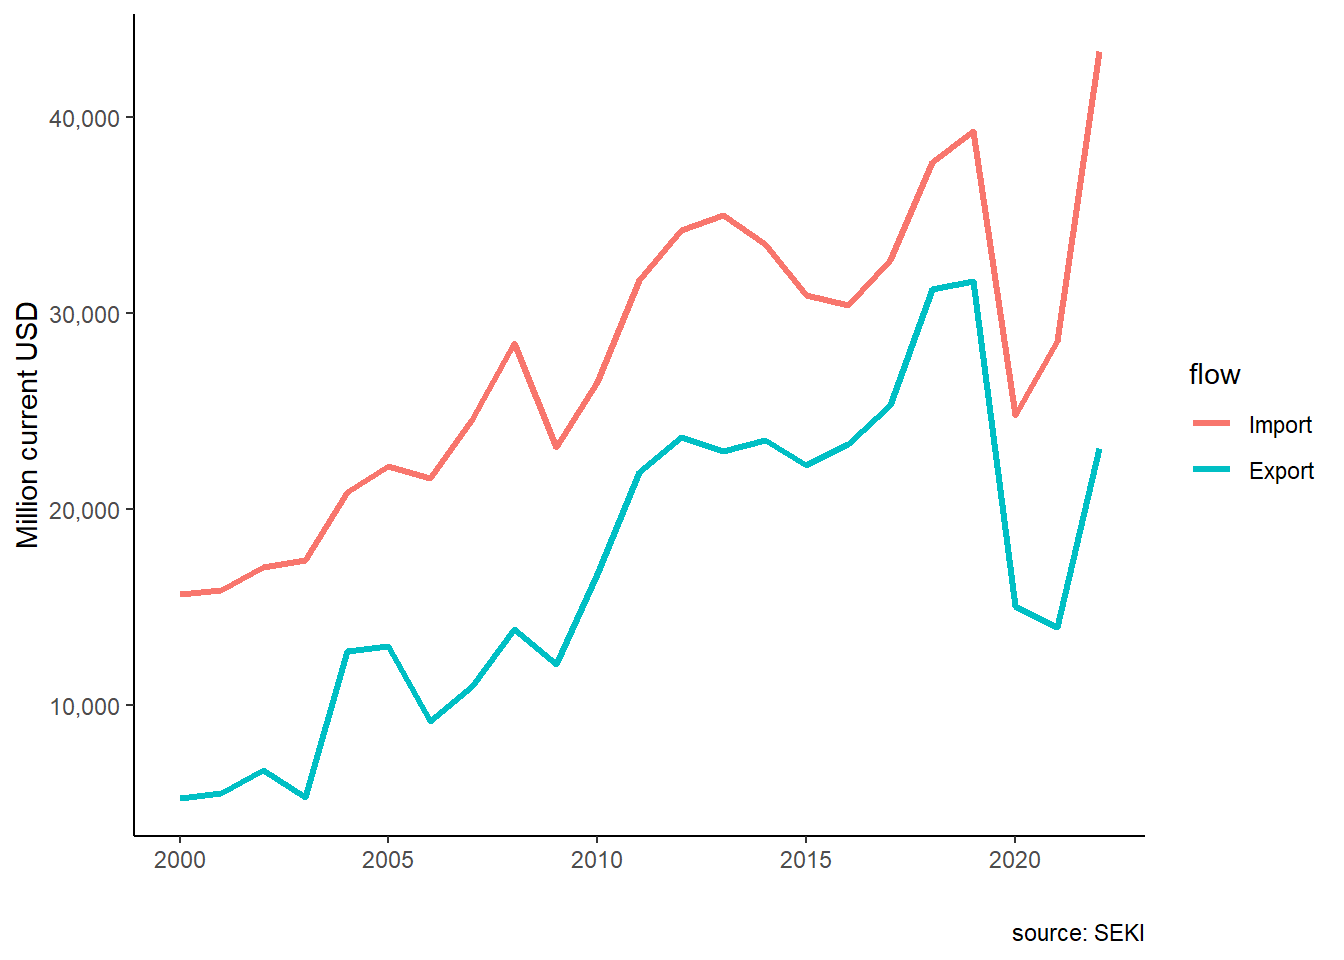
\includegraphics{plot/slides/fig1.png}

Indonesia has always been a net importer of trade. Export services is
dominated by tourism, while import services is dominated by logistics
and business services.
\end{column}

\begin{column}{0.47\textwidth}
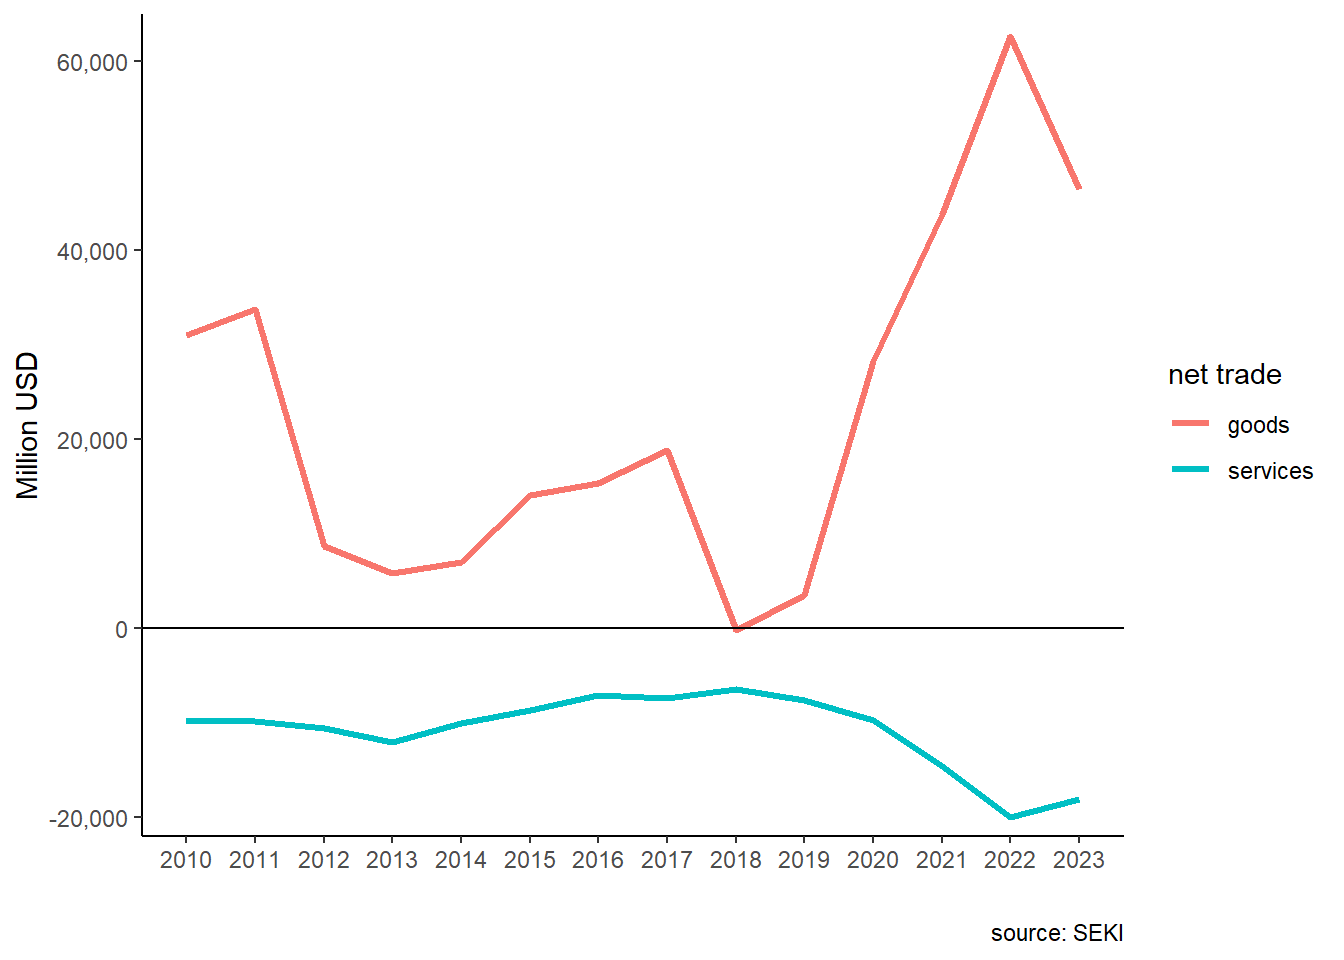
\includegraphics{plot/slides/fig2.png}

Indonesian government often concerned with deficit trade, but trade in
services has often neglected in the discussion.
\end{column}
\end{columns}
\end{frame}

\begin{frame}{But more!}
\phantomsection\label{but-more}
\begin{itemize}
\item
  With the ever decreasing cost of trade, separating a value up to tasks
  level (Baldwin, Freeman, and Theodorakopoulos 2024; Kimura 2018).
\item
  Feedback mechanism from the third unbundling may benefits domestic
  manufacturing (Kimura 2018).
\item
  In fact, exporting high-value services directly can be a good strategy
  for growth.
\end{itemize}
\end{frame}

\begin{frame}{About the chapter}
\phantomsection\label{about-the-chapter}
\begin{itemize}
\item
  The state of trade in services in Indonesia
\item
  Services as manufacturing inputs

  \begin{itemize}
  \item
    using Input-Output.
  \item
    services import-manufacturing export cointegration.
  \end{itemize}
\item
  Preliminary conclusions
\end{itemize}
\end{frame}

\begin{frame}{The third unbundling}
\phantomsection\label{the-third-unbundling}
\begin{itemize}
\item
  Unbundling: how much part of the supply chain of production can be
  traded across border increase the use of comparative advantage
  (Baldwin 2016; Kimura 2018).

  \begin{itemize}
  \tightlist
  \item
    trade cost: 1st, communication costs: 2nd, face-to-face costs: 3rd.
  \end{itemize}
\item
  3 development paths: step-by-step, leap-frogging, feedback (Kimura
  2018)
\item
  The last two makes services ever more important:

  \begin{itemize}
  \item
    leap-frog to supplying part of a services tasks, or;
  \item
    Feedback, using services to improve manufacturing.
  \end{itemize}
\end{itemize}
\end{frame}

\begin{frame}{Services in manufacturing}
\phantomsection\label{services-in-manufacturing}
\begin{itemize}
\item
  Melitz (2003): non-trivial trade cost makes small-margin firms lose.
\item
  Services can lower this cost: brigde information gap on the market,
  business customs and regulations in other countries, especially for
  new firms entering export market (Lodefalk 2014)
\item
  In Sweden, firms with higher services embeded in its final products
  increases its intensity of export (Lodefalk 2014)
\item
  In Indonesia, 10 per cent increase in service intensity of a firm
  increase its productivity by 7 to 8 per cent (Hing and Thangavelu
  2023)
\end{itemize}
\end{frame}

\begin{frame}{Services trade in Indonesia}
\phantomsection\label{services-trade-in-indonesia}
\begin{itemize}
\item
  Trade in services is complicated amid 4 modes (Magiera 2011):

  \begin{itemize}
  \item
    mode 2 \& 4 \(\rightarrow\) Visa and KITAS regulations
  \item
    mode 3 \(\rightarrow\) investment and operational.
  \end{itemize}
\item
  Magiera (2011): complicated authorities, unlike goods. Makes it hard
  to discuss Deep Trade Agreements (Syahputri and Gupta 2024).
\item
  IJEPA: no evidence it improves services trade (Syahputri and Gupta
  2024)
\end{itemize}
\end{frame}

\begin{frame}{Data: BaTIS}
\phantomsection\label{data-batis}
\begin{columns}[T]
\begin{column}{0.47\textwidth}
\begin{itemize}
\item
  First launched in 2017 by OECD and WTO (Liberatore and Wettstein
  2021),
\item
  Balanced data from two trading partners.
\item
  Not very good outside of rich countries.
\item
  used to build other databases like TiVA.
\end{itemize}
\end{column}

\begin{column}{0.47\textwidth}
\begin{longtable}[]{@{}ll@{}}
\caption{Services classification in BaTIS}\label{tbl-1}\tabularnewline
\toprule\noalign{}
Code & Category description \\
\midrule\noalign{}
\endfirsthead
\toprule\noalign{}
Code & Category description \\
\midrule\noalign{}
\endhead
SA & Manufacturing services on physical inputs owned by others \\
SB & Maintenance and repair services n.i.e. \\
SC & Transport \\
SD & Travel \\
SE & Construction \\
SF & Insurance and pension services \\
SG & Financial services \\
SH & Charges for the use of intellectual property n.i.e. \\
SI & Telecommunications, computer, and information services \\
SJ & Other business services \\
SK & Personal, cultural and recreational services \\
SL & Government goods and services n.i.e. \\
\bottomrule\noalign{}
\end{longtable}
\end{column}
\end{columns}
\end{frame}

\begin{frame}{Trade by partner,2021}
\phantomsection\label{trade-by-partner2021}
\begin{columns}[T]
\begin{column}{0.47\textwidth}
\begin{figure}

\centering{

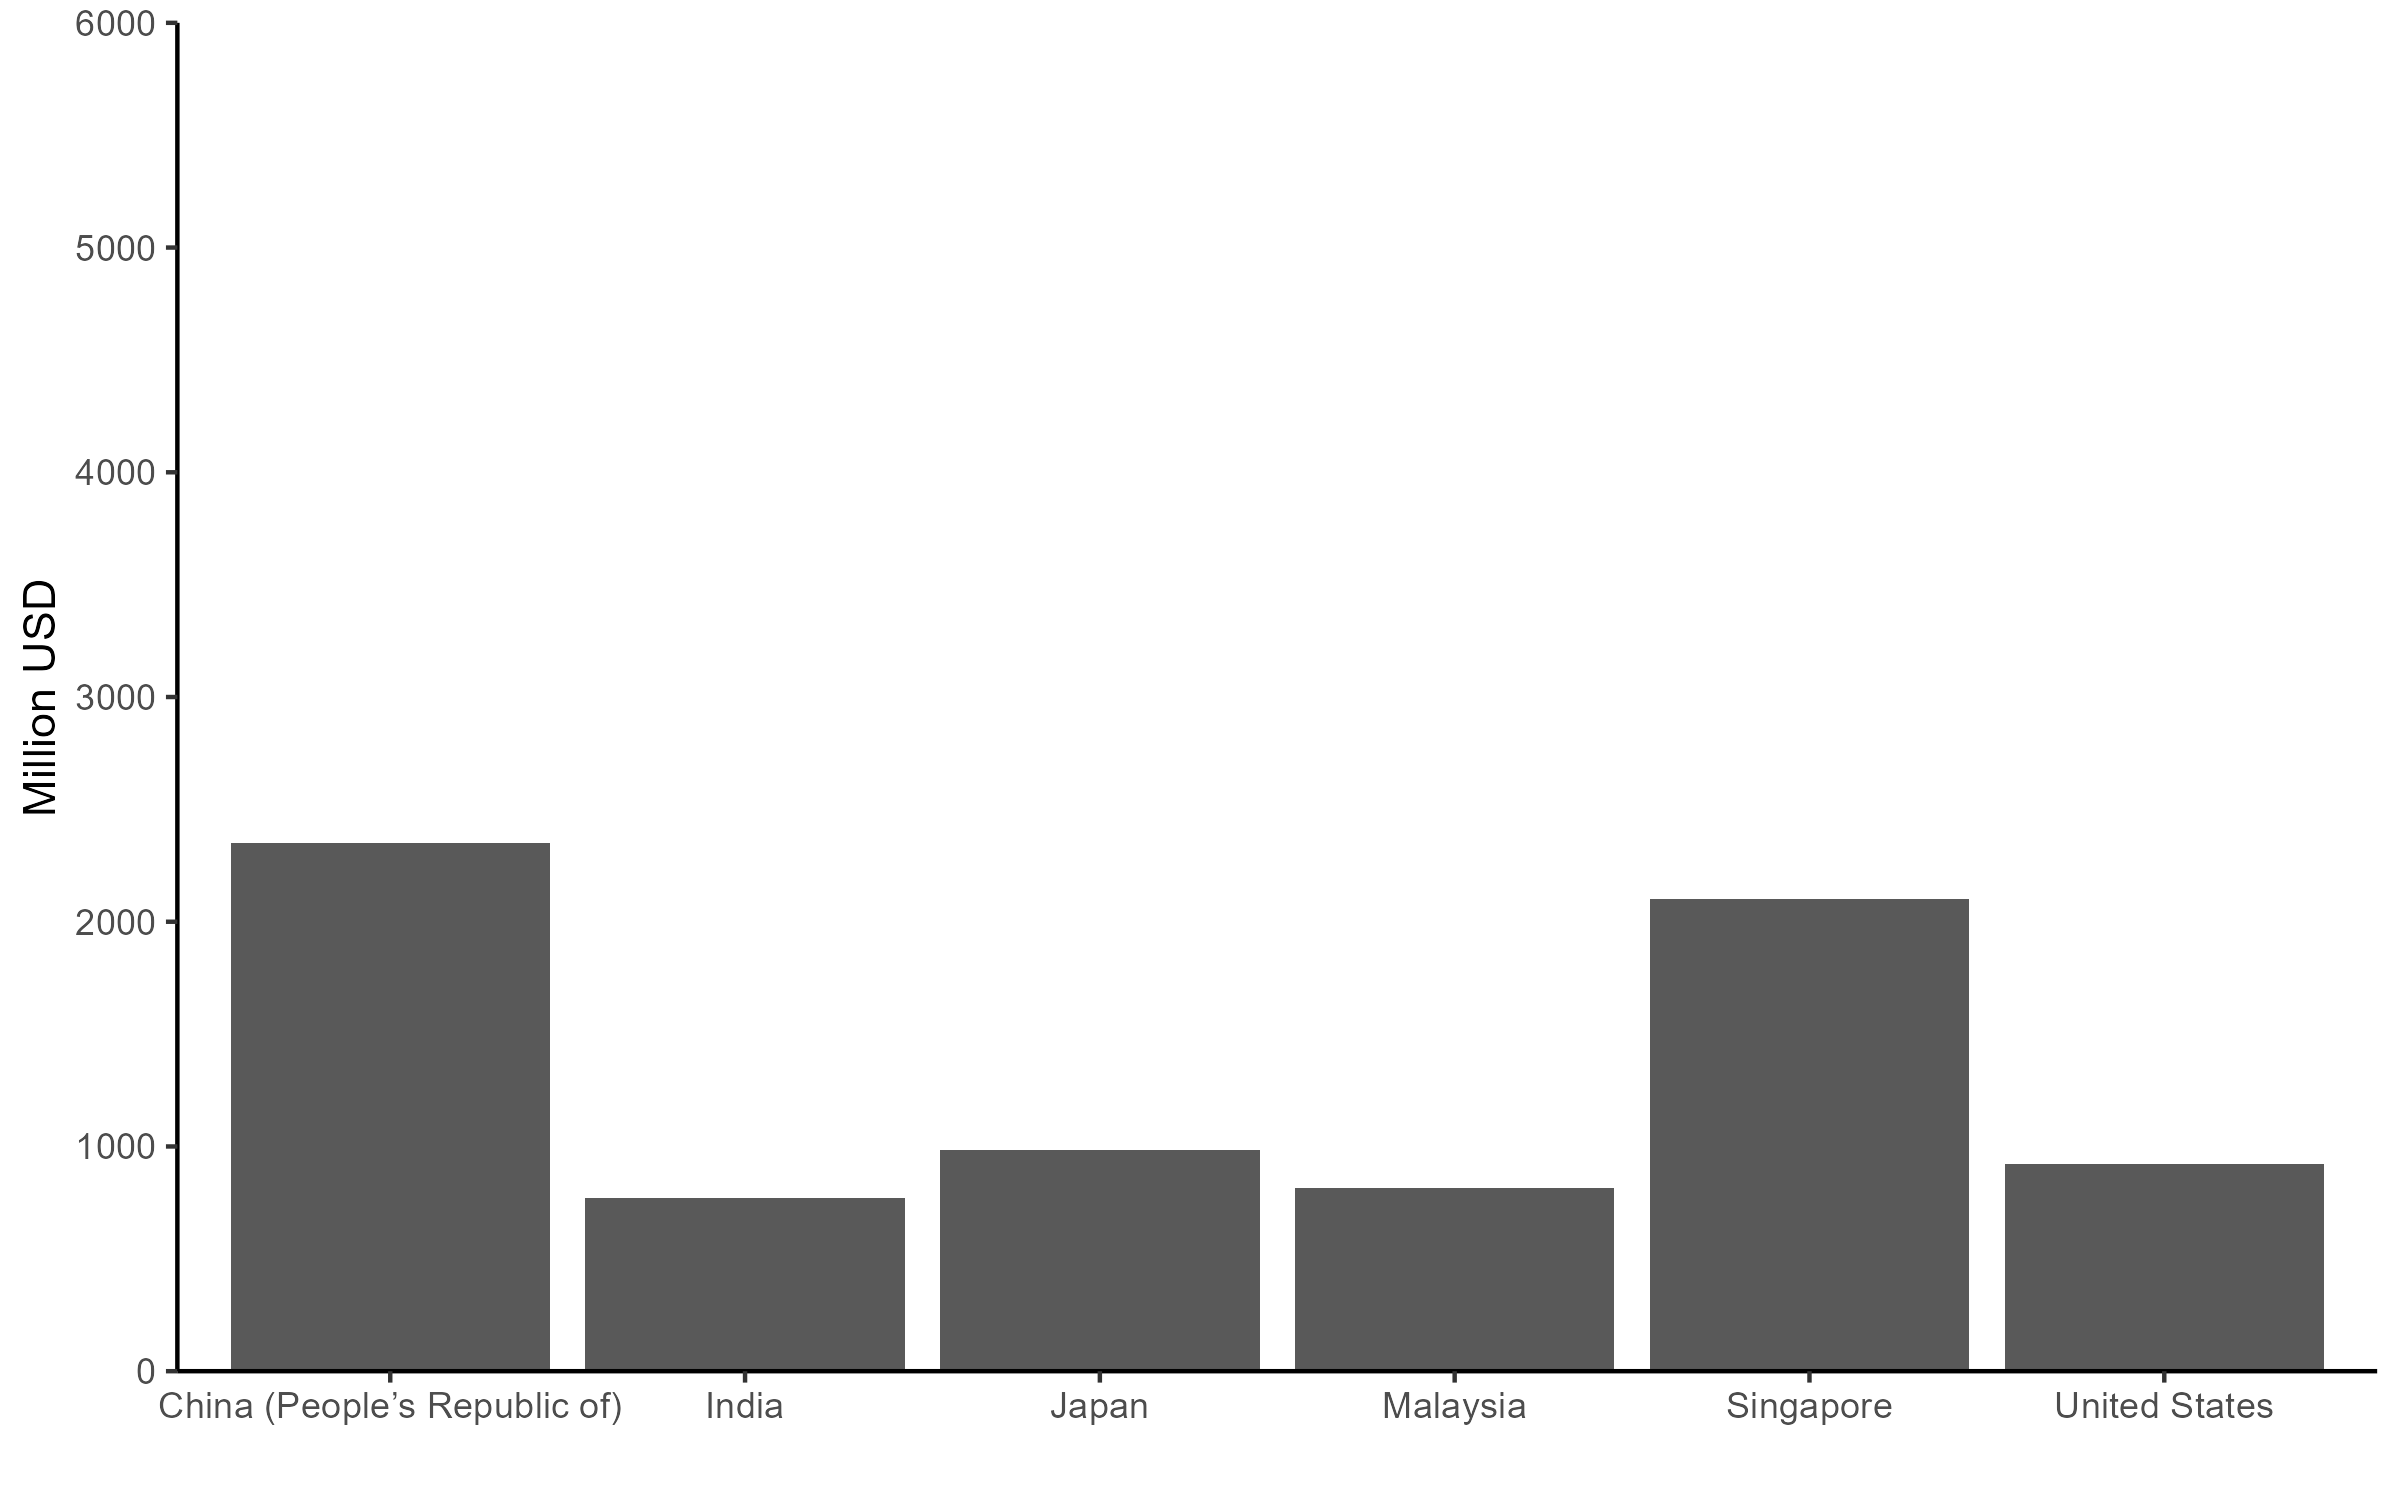
\includegraphics{plot/allcx.png}

}

\caption{\label{fig-CX}Indonesia's exports by partner, 2021}

\end{figure}%
\end{column}

\begin{column}{0.47\textwidth}
\begin{figure}

\centering{

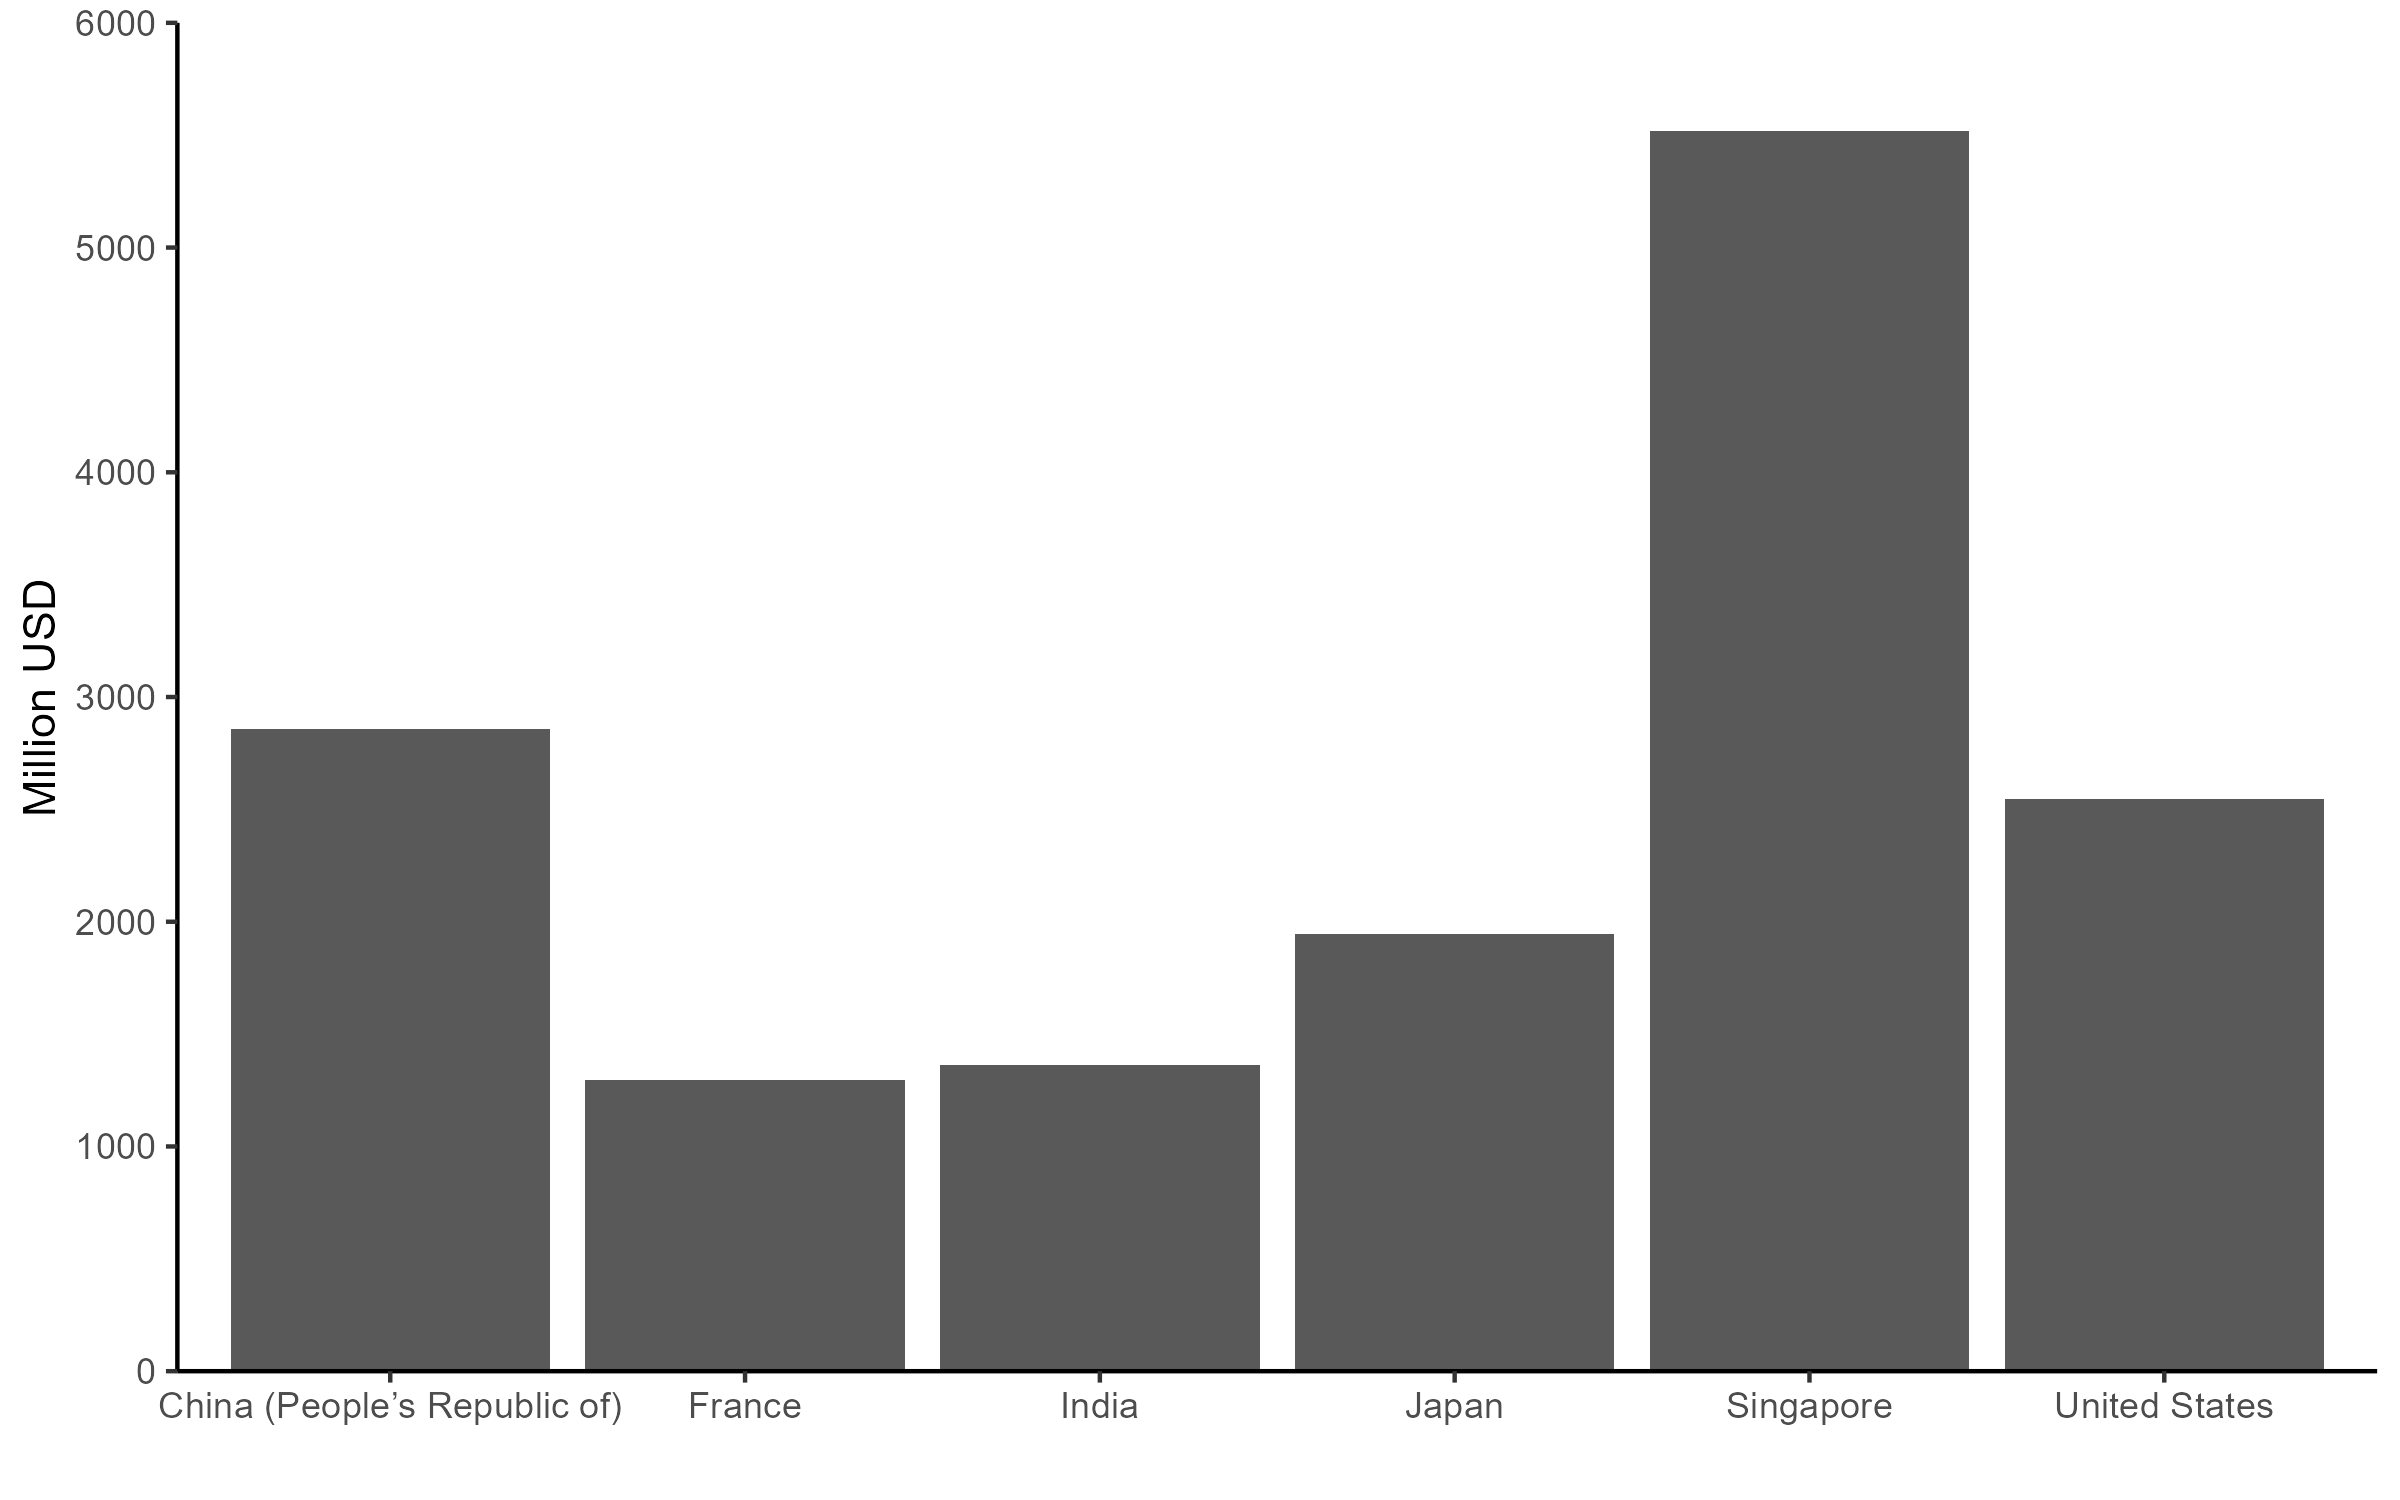
\includegraphics{plot/allcm.png}

}

\caption{\label{fig-CM}Indonesia's imports by partner, 2021}

\end{figure}%
\end{column}
\end{columns}

Singapore is the most important partner in trade in services for
Indonesia. China, on the other hand, is the main buyer of Indonesia's
services export
\end{frame}

\begin{frame}{Trade by sector, 2021}
\phantomsection\label{trade-by-sector-2021}
\begin{columns}[T]
\begin{column}{0.47\textwidth}
\begin{figure}

\centering{

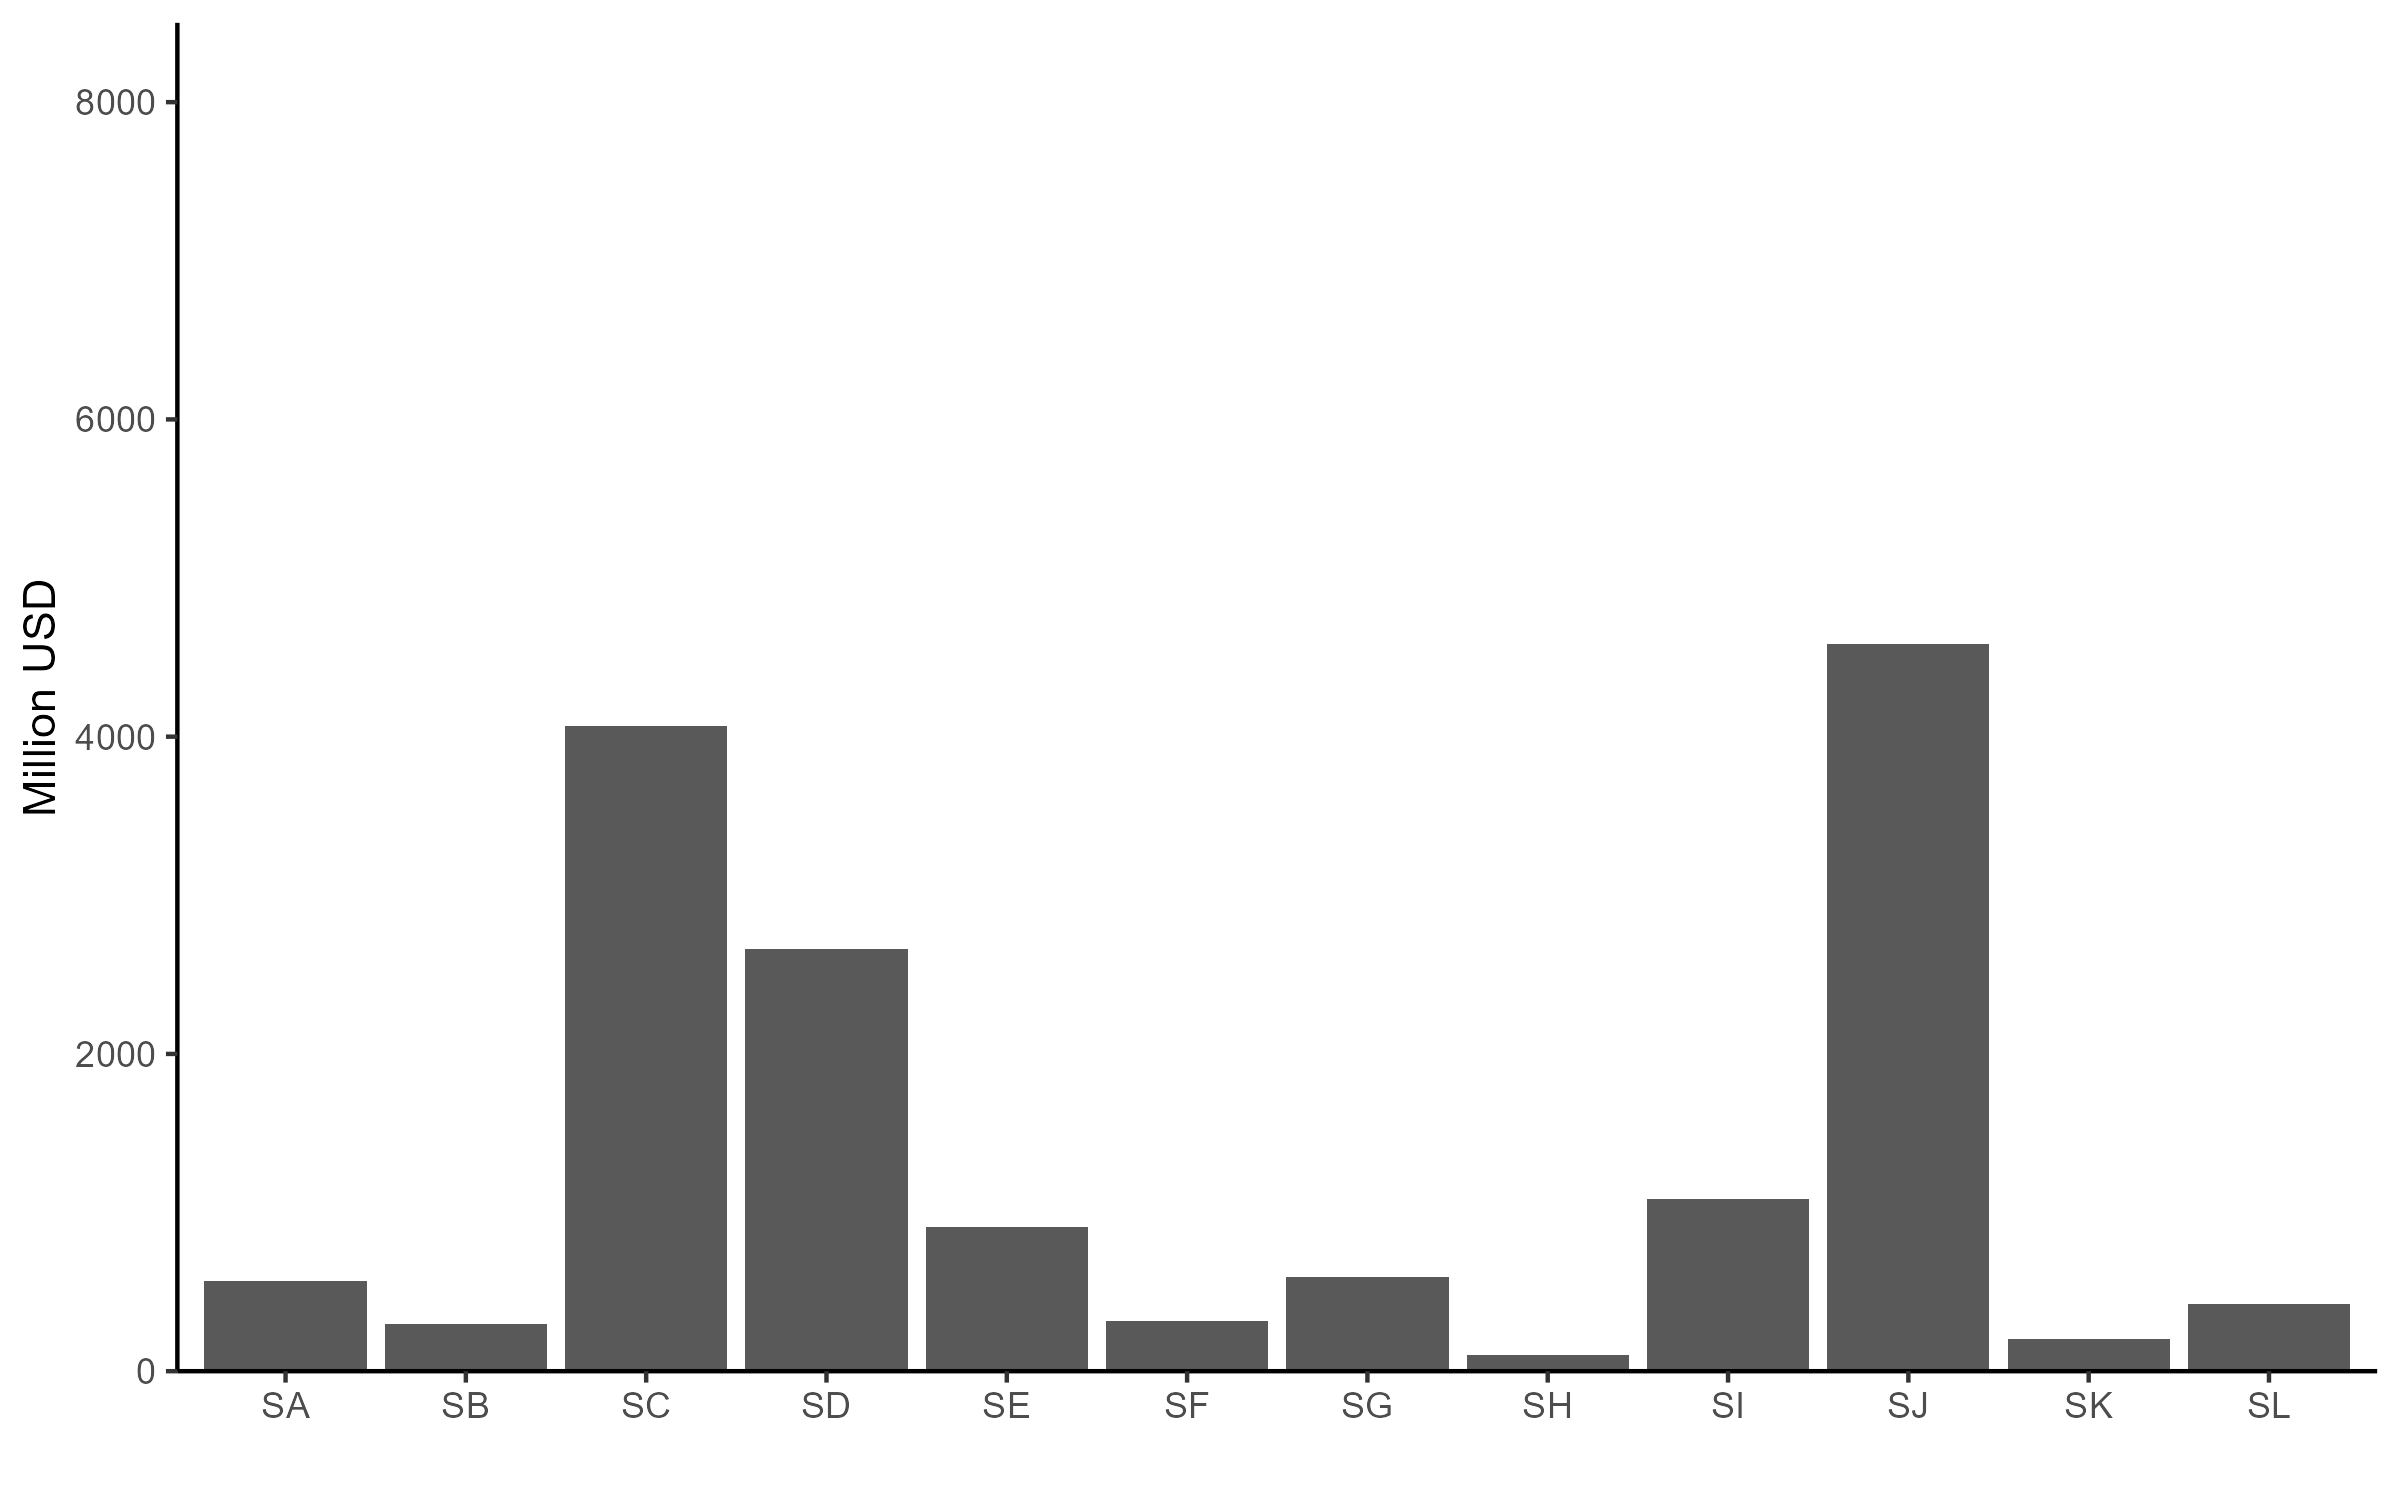
\includegraphics{plot/allsx.png}

}

\caption{\label{fig-SX}Indonesia's exports by sector, 2021}

\end{figure}%
\end{column}

\begin{column}{0.47\textwidth}
\begin{figure}

\centering{

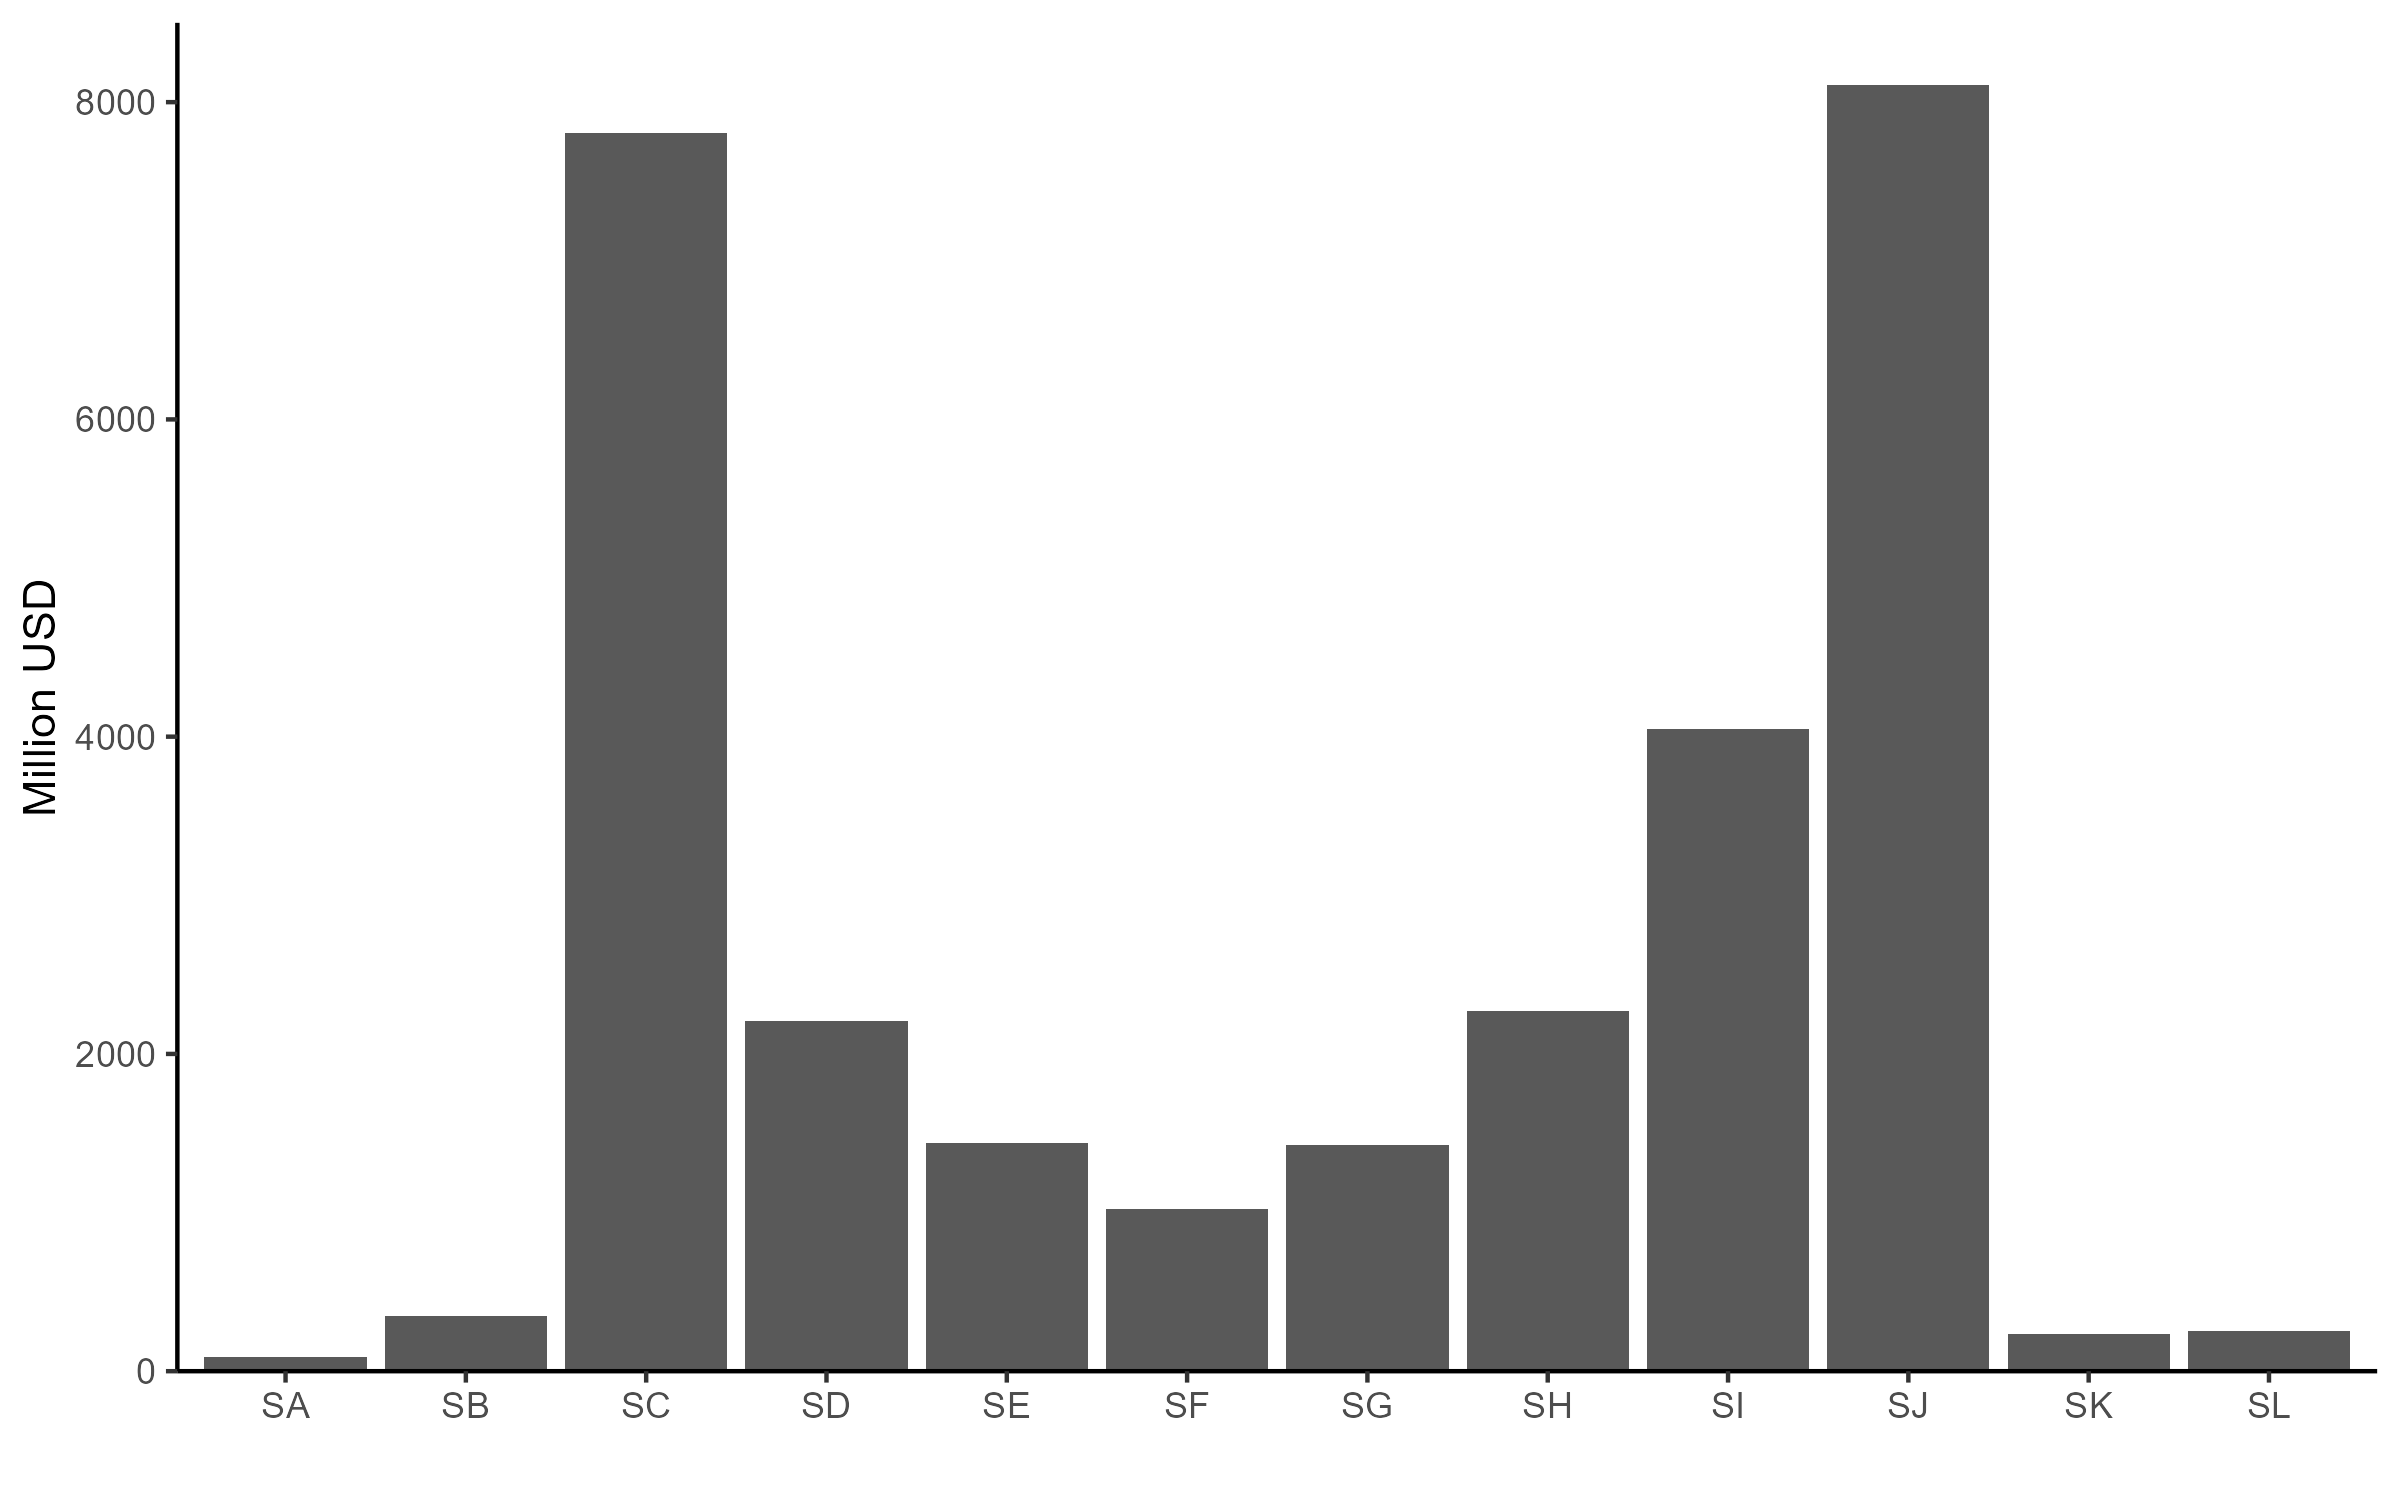
\includegraphics{plot/allsm.png}

}

\caption{\label{fig-SM}Indonesia's imports by sector, 2021}

\end{figure}%
\end{column}
\end{columns}

Indonesia's imports dominates exports in all categories bar travel (SD).
Additionally, the highest traded services in Indonesia are transport
(SC) and business services (SJ)
\end{frame}

\begin{frame}{Top services: travel}
\phantomsection\label{top-services-travel}
\begin{columns}[T]
\begin{column}{0.47\textwidth}
\begin{figure}

\centering{

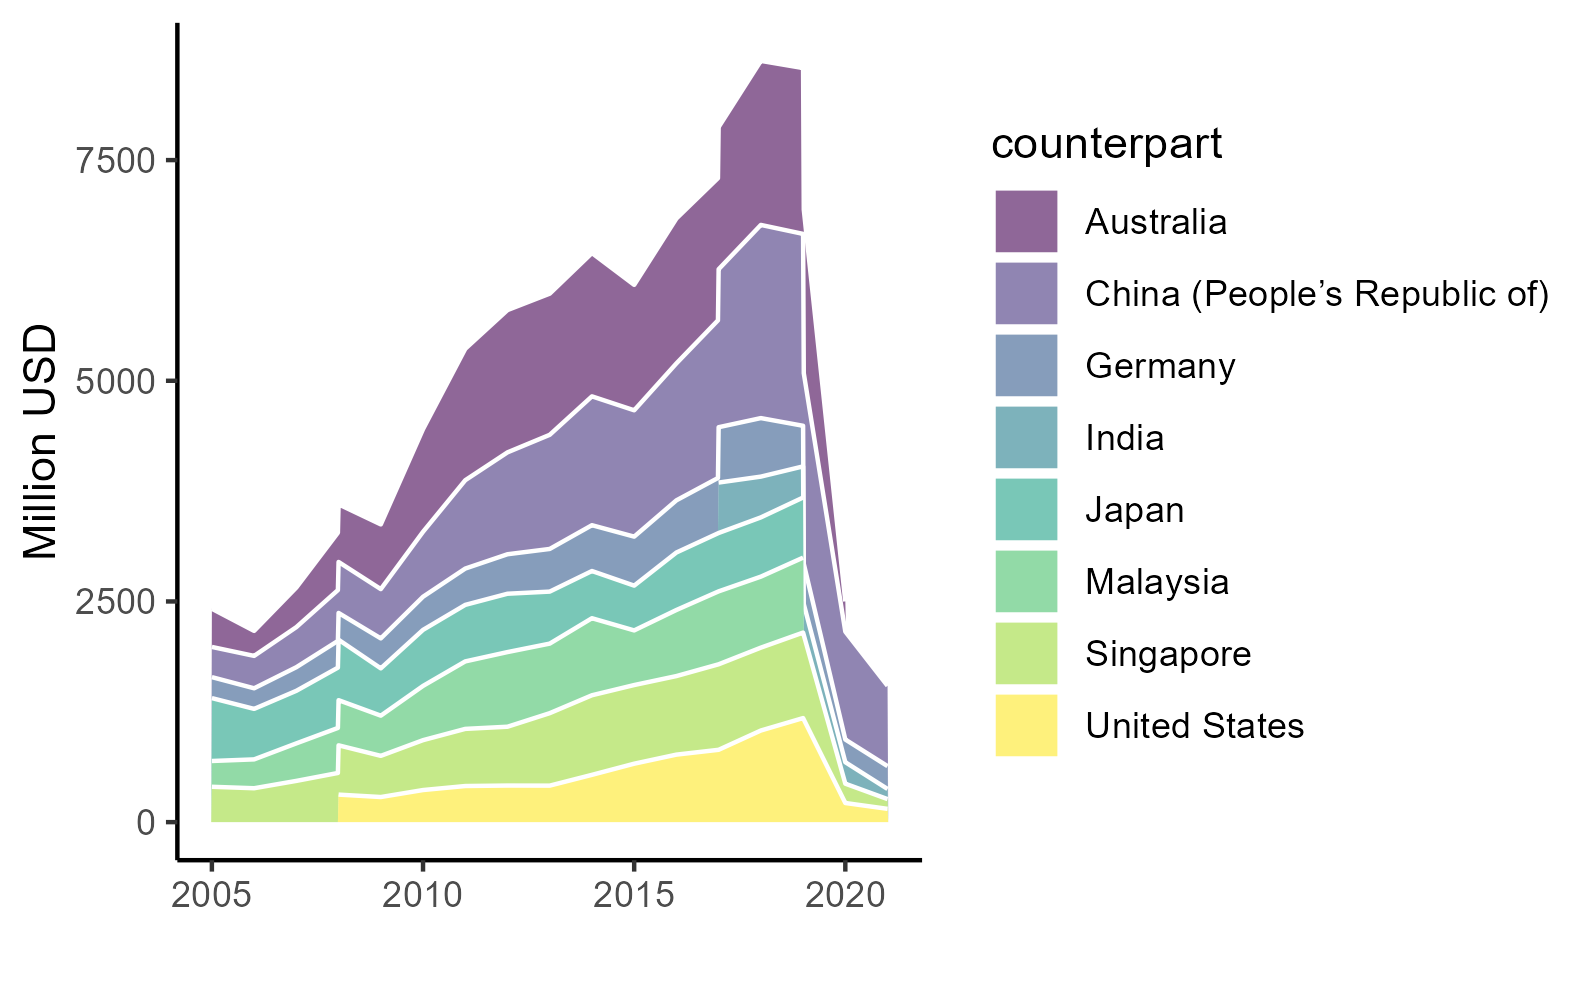
\includegraphics{plot/SDEX.png}

}

\caption{\label{fig-SX}Indonesia's travel export, top 6 partners}

\end{figure}%
\end{column}

\begin{column}{0.47\textwidth}
\begin{figure}

\centering{

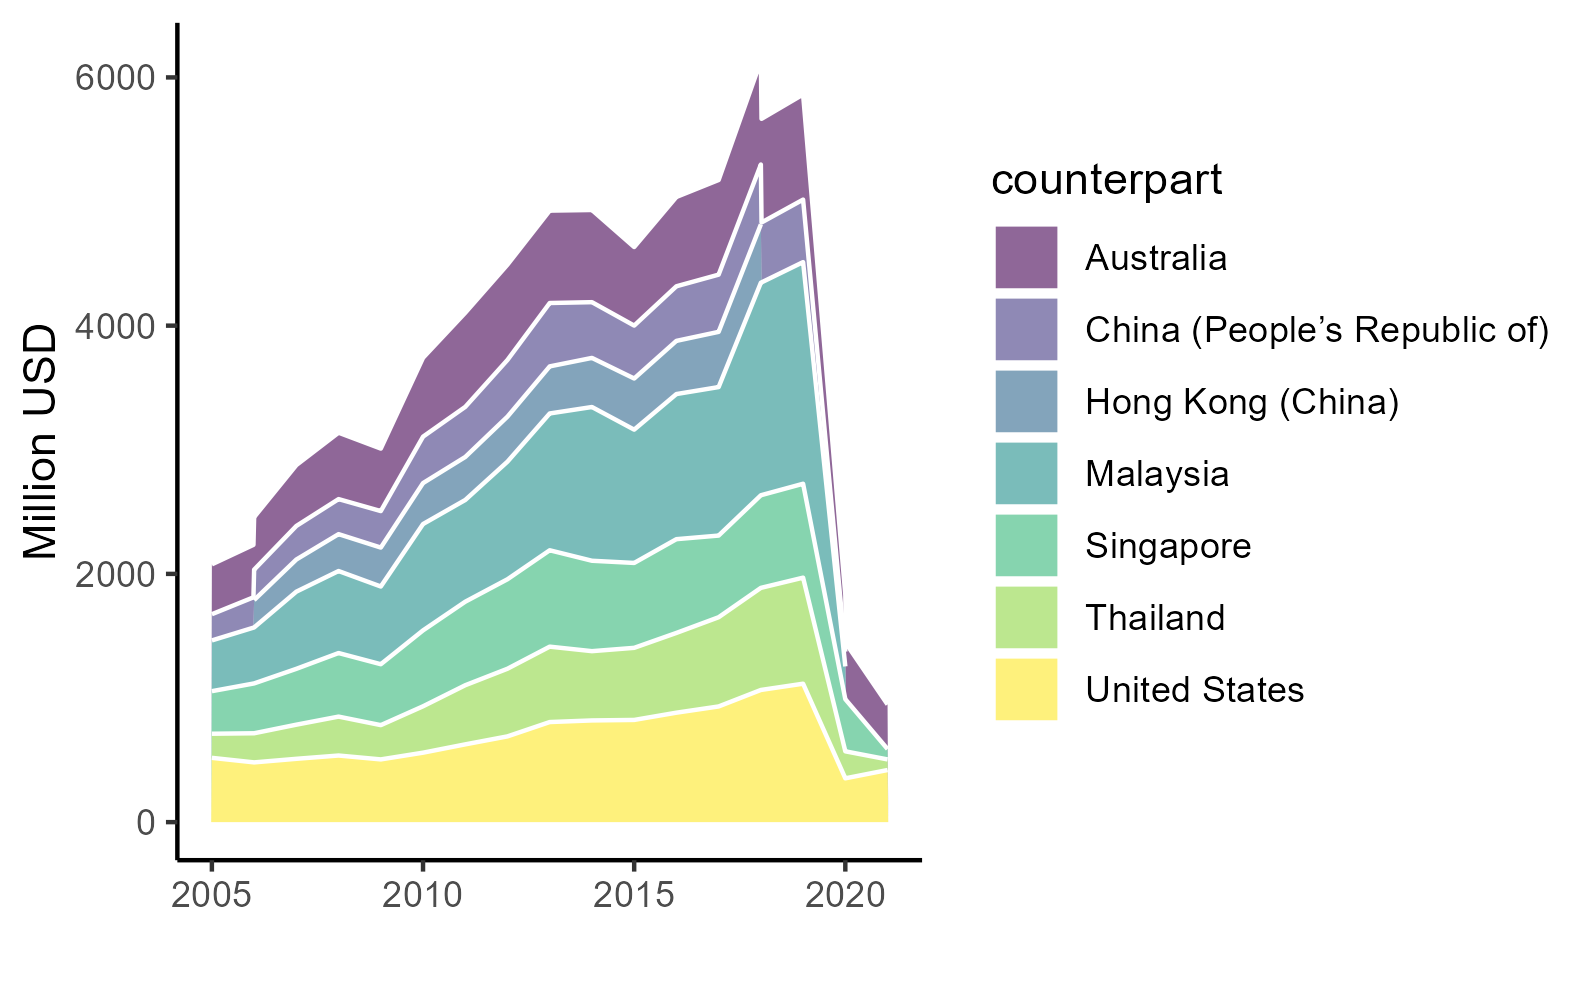
\includegraphics{plot/SDIM.png}

}

\caption{\label{fig-SM}Indonesia's travel import, top 6 partners}

\end{figure}%
\end{column}
\end{columns}

The only net export got punished by the pandemic. China+Australia
important export destination,
\end{frame}

\begin{frame}{Top services: transport}
\phantomsection\label{top-services-transport}
\begin{columns}[T]
\begin{column}{0.47\textwidth}
\begin{figure}

\centering{

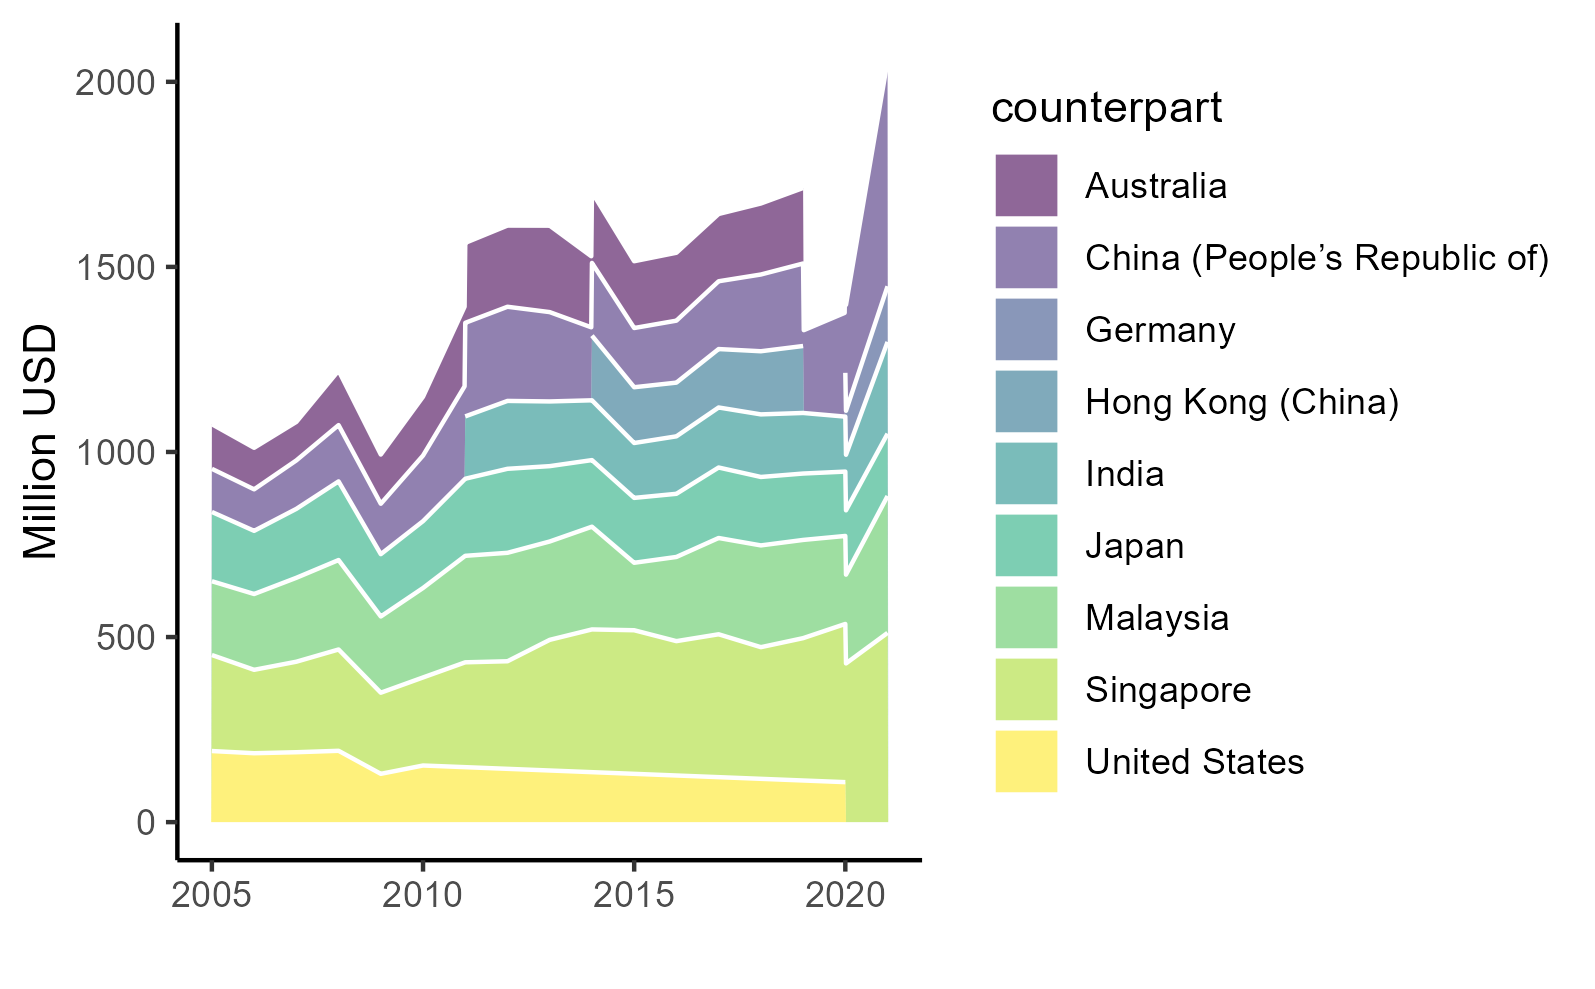
\includegraphics{plot/SCEX.png}

}

\caption{\label{fig-SX}Indonesia's travel export, top 6 partners}

\end{figure}%
\end{column}

\begin{column}{0.47\textwidth}
\begin{figure}

\centering{

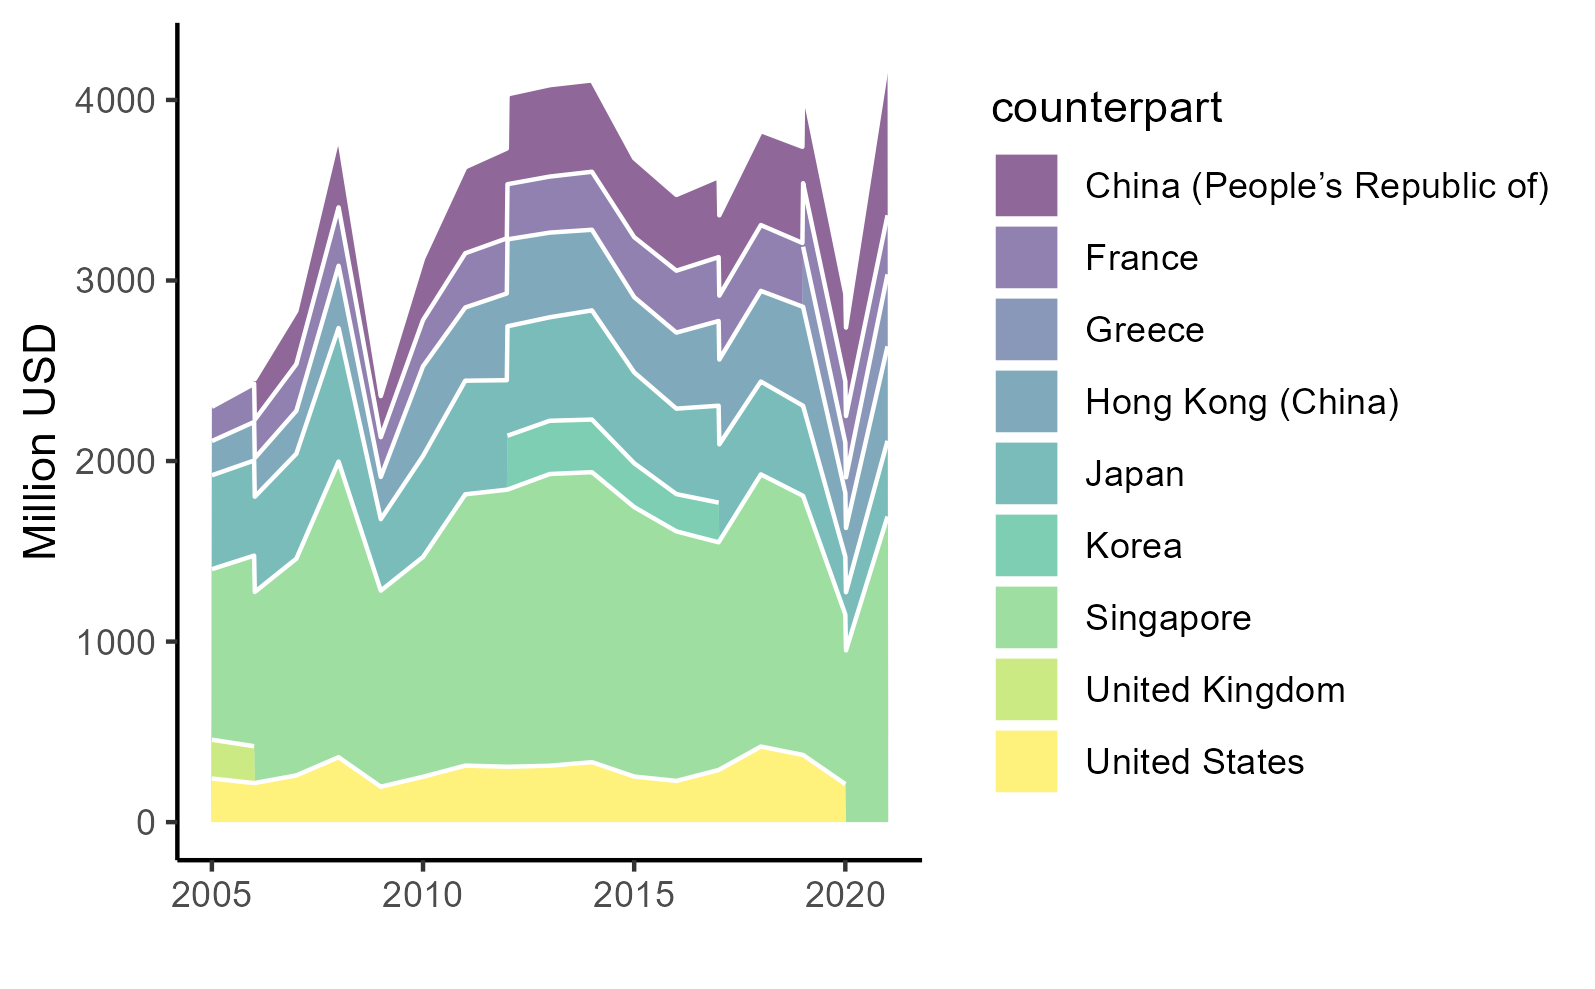
\includegraphics{plot/SCIM.png}

}

\caption{\label{fig-SM}Indonesia's travel import, top 6 partners}

\end{figure}%
\end{column}
\end{columns}

Singapore's dominance is apparent here. Very important for manufactures
trade.
\end{frame}

\begin{frame}{Top services: ICT services}
\phantomsection\label{top-services-ict-services}
\begin{columns}[T]
\begin{column}{0.47\textwidth}
\begin{figure}

\centering{

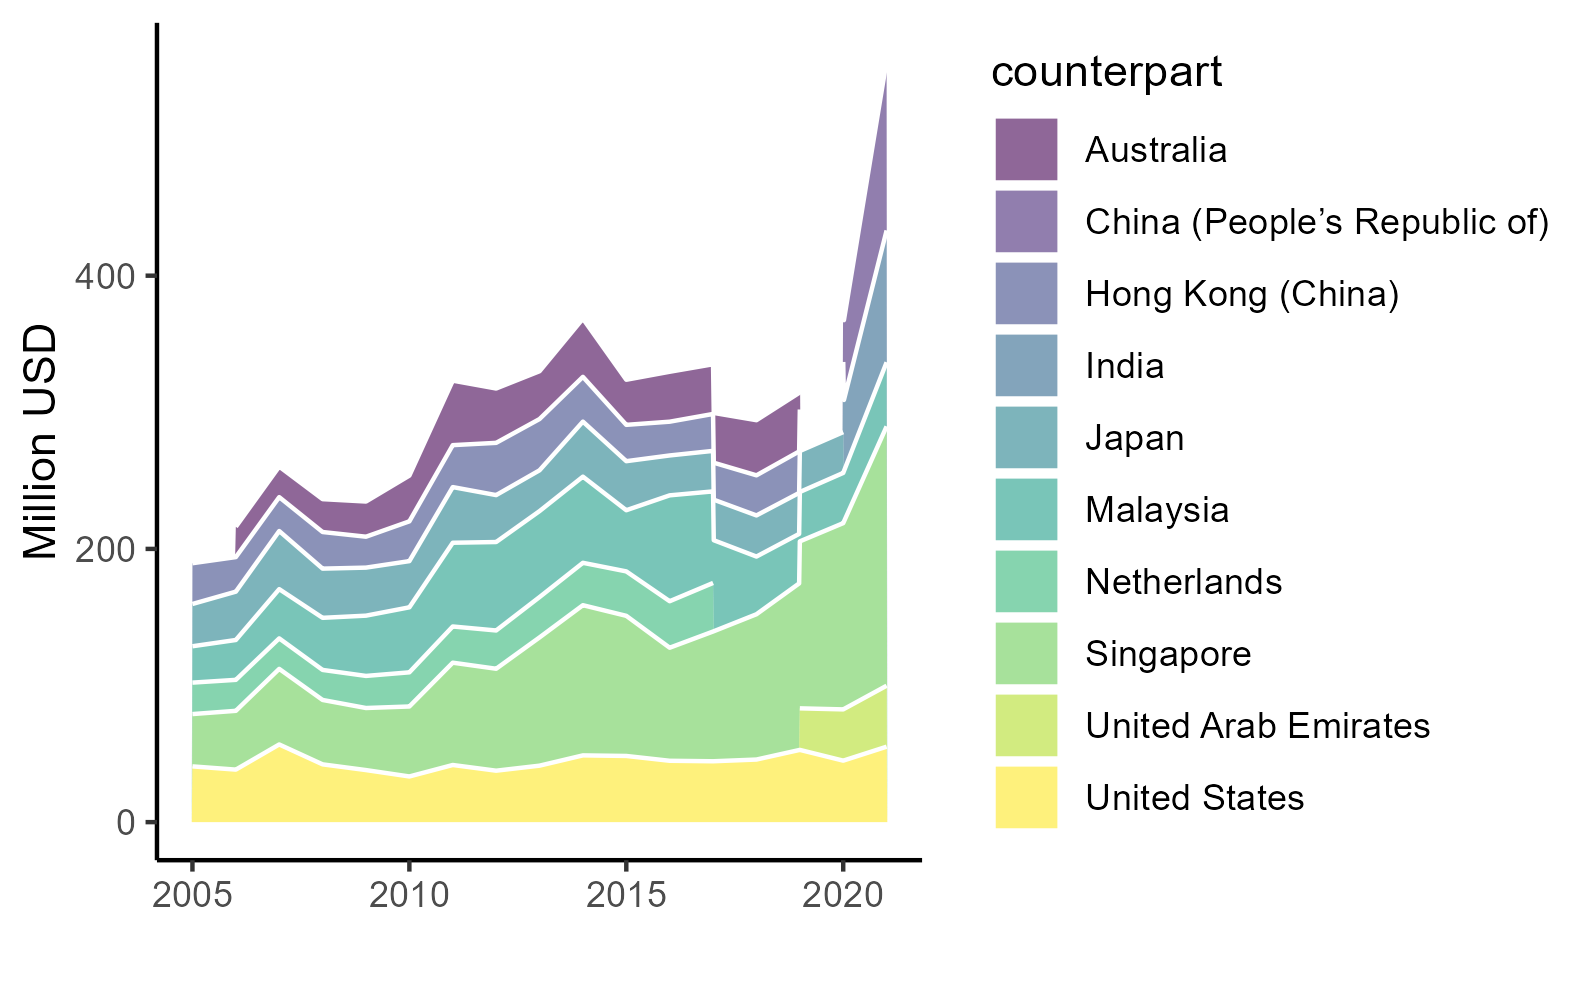
\includegraphics{plot/SIEX.png}

}

\caption{\label{fig-SX}Indonesia's ICT service export, top 6 partners}

\end{figure}%
\end{column}

\begin{column}{0.47\textwidth}
\begin{figure}

\centering{

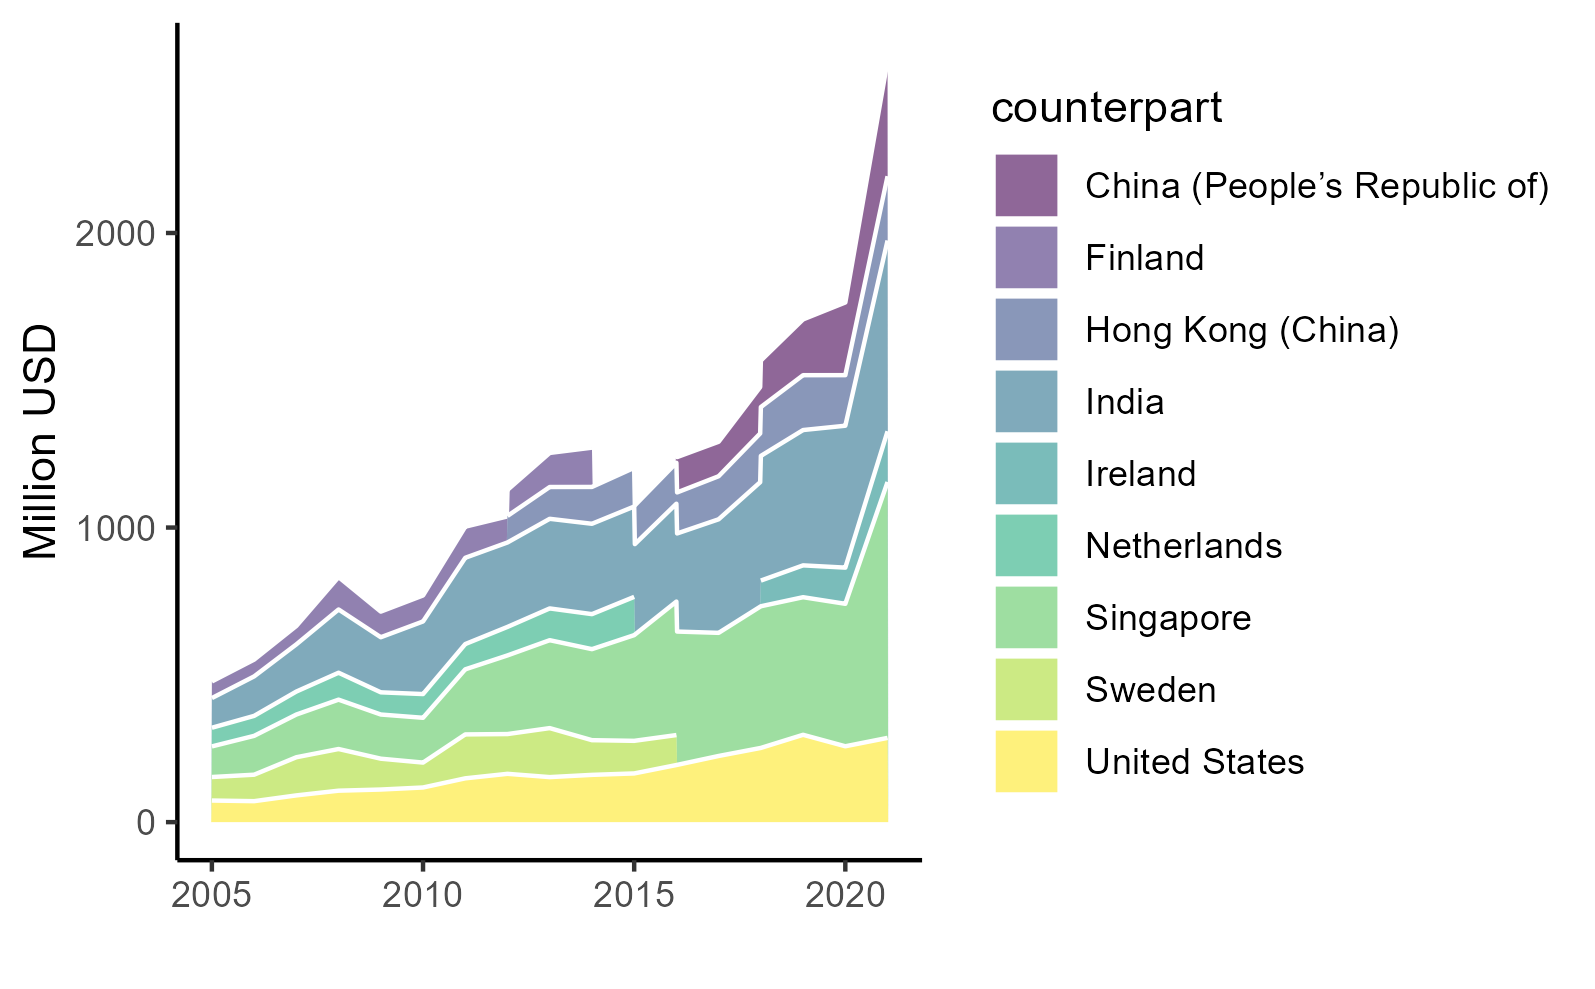
\includegraphics{plot/SIIM.png}

}

\caption{\label{fig-SM}Indonesia's ICT service import, top 6 partners}

\end{figure}%
\end{column}
\end{columns}

Perhaps the most relevant services to leap-frogging and feedback. Also
the highest beneficiary of the pandemic.
\end{frame}

\begin{frame}{Top services: biz services}
\phantomsection\label{top-services-biz-services}
\begin{columns}[T]
\begin{column}{0.47\textwidth}
\begin{figure}

\centering{

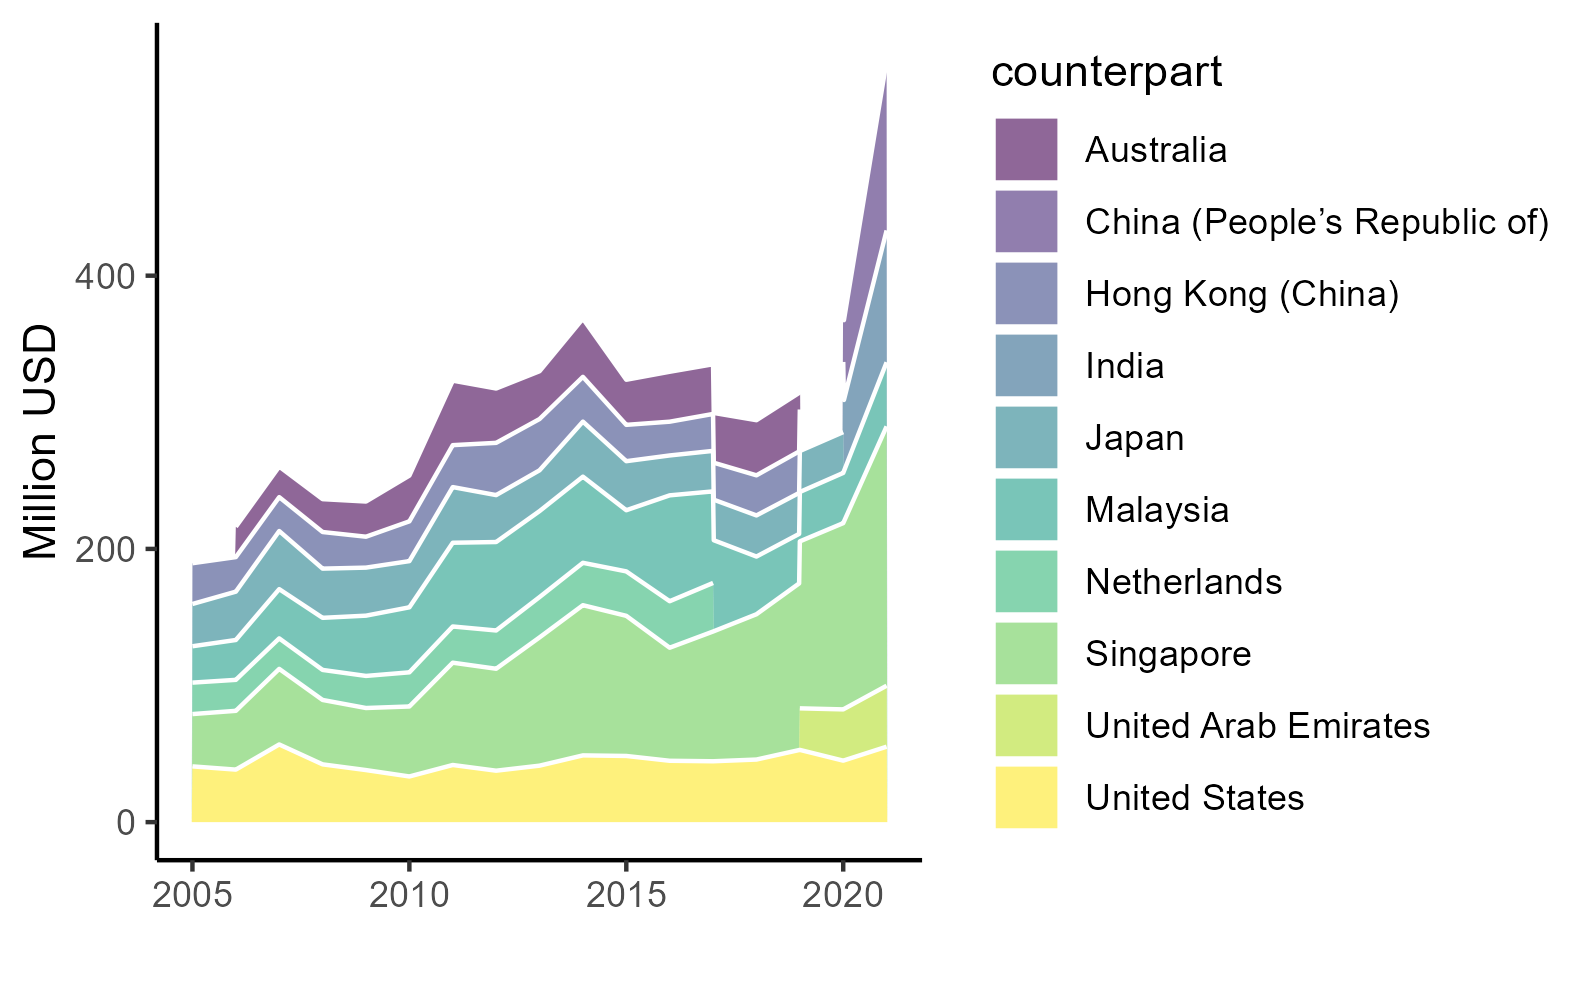
\includegraphics{plot/SIEX.png}

}

\caption{\label{fig-SX}Indonesia's ICT service export, top 6 partners}

\end{figure}%
\end{column}

\begin{column}{0.47\textwidth}
\begin{figure}

\centering{

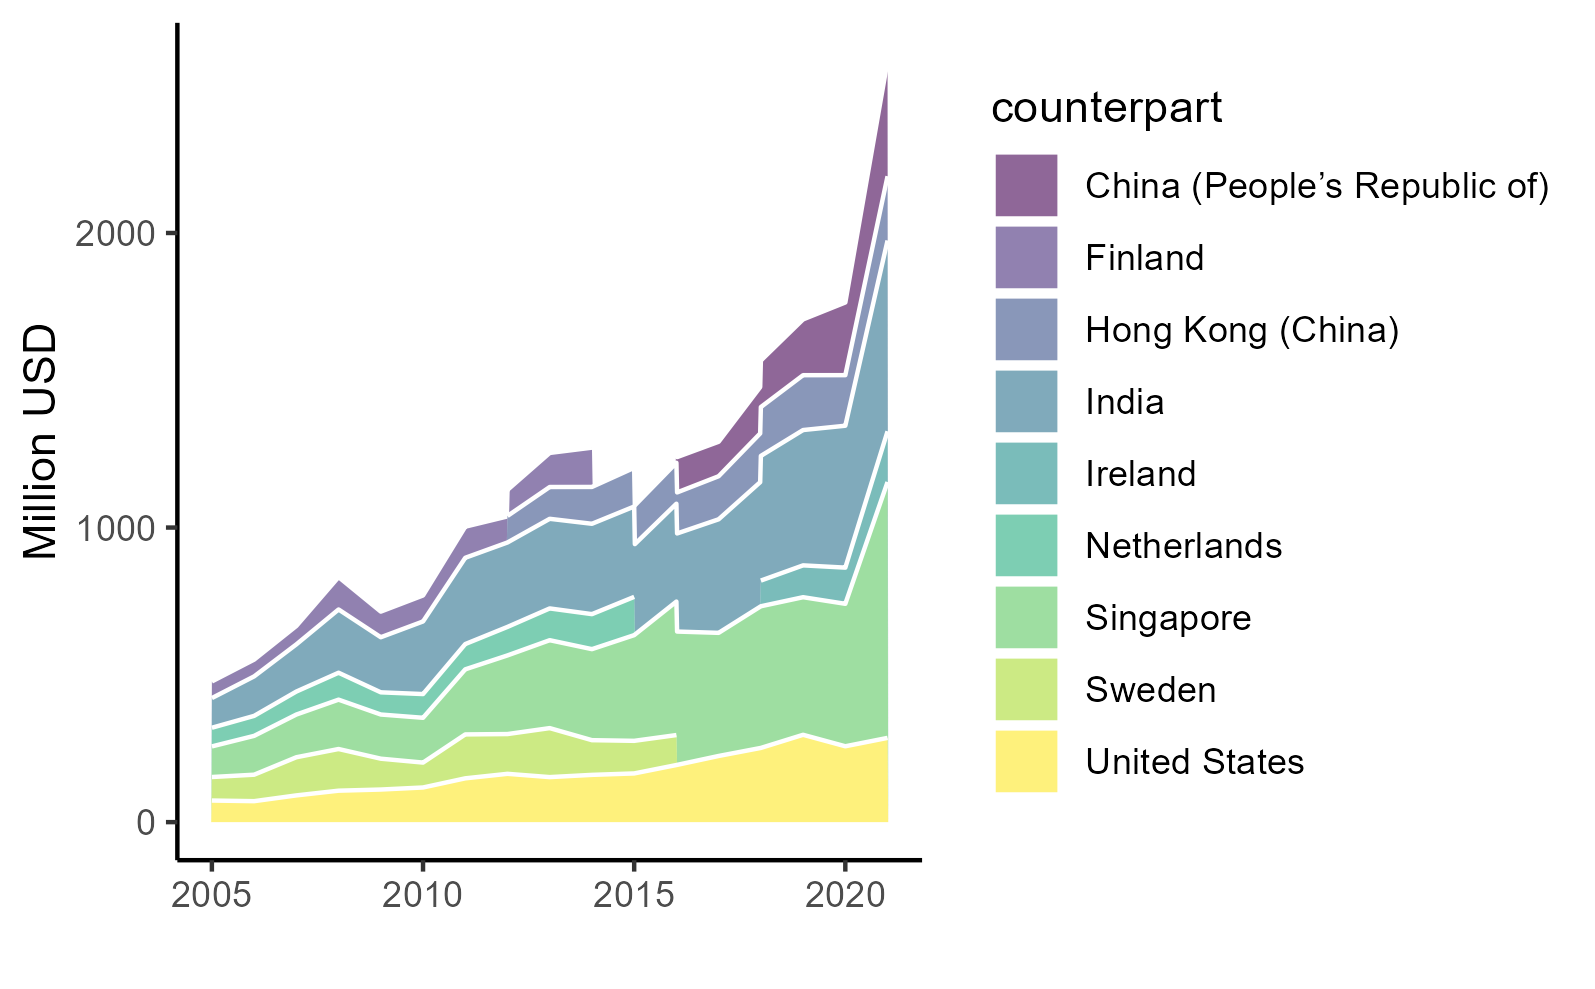
\includegraphics{plot/SIIM.png}

}

\caption{\label{fig-SM}Indonesia's ICT service import, top 6 partners}

\end{figure}%
\end{column}
\end{columns}

Other business services includes consulting management, research and
development, and trade-related services (Liberatore et al. 2021)
\end{frame}

\begin{frame}{All in all}
\phantomsection\label{all-in-all}
\begin{itemize}
\item
  Singapore is important for Indonesia
\item
  Travel carry the trade balance. Most travel exports comes mainly from
  tourism, which is bad since the pandemic punishes it
  disproportionately.
\item
  Trade agreements play a huge role in improving trade in services.
\item
  Measures that affects movement of natural persons (e.g., qualification
  harmonization), and other non-tariff measures like computing
  requirement and investment list are crucial as trade in services can
  be done in 4 different modes that got affected by these rules.
\end{itemize}
\end{frame}

\begin{frame}{Manufacturing feedback}
\phantomsection\label{manufacturing-feedback}
\begin{itemize}
\item
  We look at the role of imported services to Indonesian manufacturing,
  a sector Indonesian government tries to revive for a long time.
\item
  Two approaches: input-output table and ARDL cointegration.
\item
  Input-Output utilises ICIO data (OECD 2023), the ARDL uses Indonesian
  Central Bank data (Bank Indonesia, n.d.)
\end{itemize}
\end{frame}

\begin{frame}{ICIO}
\phantomsection\label{icio}
Let there be a nest of product from some degree of substitutable
services input:

\[
Y_{it}=f(AS^D_{it},AS^F_{it})
\]

for all \(i=\) manufacturing sectors and \(t=year\). A is the nest
multiplier, \(S^D_i\) and \(S^F_i\) are total services purchased by
industry \(i\), domestically and imported respectively.

Assuming a Cobb-Douglass relationship, a log-linearized version thus

\[
y_{it}=a+\beta_d s^D_{it}+\beta_f s^F_{it}+\varepsilon_{it}
\]
\end{frame}

\begin{frame}{ICIO}
\phantomsection\label{icio-1}
To construct the dataset for the regression, we aggregate non-factor
inputs from each manufacuring sectors, separated by whether it is from
Indonesia or from other countries. All inputs from foreign countries are
aggregated into foreign.

For comparison purpose, we also do the same for 4 countries in the
region, namely Singapore, Malaysia, Thailand and Vietnam. Data from
these 5 countries are then concatenated to add one more dimension,
countries. Summary statistics on the data is shown in
Table~\ref{tbl-icio}.
\end{frame}

\begin{frame}{Summary}
\phantomsection\label{summary}
\begin{longtable}[]{@{}
  >{\raggedright\arraybackslash}p{(\columnwidth - 12\tabcolsep) * \real{0.2292}}
  >{\raggedright\arraybackslash}p{(\columnwidth - 12\tabcolsep) * \real{0.1146}}
  >{\raggedright\arraybackslash}p{(\columnwidth - 12\tabcolsep) * \real{0.1146}}
  >{\raggedright\arraybackslash}p{(\columnwidth - 12\tabcolsep) * \real{0.1250}}
  >{\raggedright\arraybackslash}p{(\columnwidth - 12\tabcolsep) * \real{0.1146}}
  >{\raggedright\arraybackslash}p{(\columnwidth - 12\tabcolsep) * \real{0.1146}}
  >{\raggedright\arraybackslash}p{(\columnwidth - 12\tabcolsep) * \real{0.1354}}@{}}

\caption{\label{tbl-icio}Summary Statistics from ICIO, million USD,
2002-2021.}

\tabularnewline

\toprule\noalign{}
\begin{minipage}[b]{\linewidth}\raggedright
\end{minipage} &
\multicolumn{3}{>{\raggedright\arraybackslash}p{(\columnwidth - 12\tabcolsep) * \real{0.3542} + 4\tabcolsep}}{%
\begin{minipage}[b]{\linewidth}\raggedright
all
\end{minipage}} &
\multicolumn{3}{>{\raggedright\arraybackslash}p{(\columnwidth - 12\tabcolsep) * \real{0.3646} + 4\tabcolsep}@{}}{%
\begin{minipage}[b]{\linewidth}\raggedright
IDN
\end{minipage}} \\
\begin{minipage}[b]{\linewidth}\raggedright
\end{minipage} & \begin{minipage}[b]{\linewidth}\raggedright
Mean
\end{minipage} & \begin{minipage}[b]{\linewidth}\raggedright
SD
\end{minipage} & \begin{minipage}[b]{\linewidth}\raggedright
Histogram
\end{minipage} & \begin{minipage}[b]{\linewidth}\raggedright
Mean
\end{minipage} & \begin{minipage}[b]{\linewidth}\raggedright
SD
\end{minipage} & \begin{minipage}[b]{\linewidth}\raggedright
Histogram
\end{minipage} \\
\midrule\noalign{}
\endhead
\bottomrule\noalign{}
\endlastfoot
value added & 4181.70 & 6845.40 & ▇▁ & 8150.56 & 12191.95 & ▇▁ \\
output & 15930.67 & 21741.55 & ▇▁ & 21529.33 & 29317.48 & ▇▁▁ \\
domestic services & 2804.36 & 3889.86 & ▇▂▁ & 3735.21 & 4176.07 & ▇▅▁ \\
foreign services & 845.74 & 1730.29 & ▇ & 420.05 & 339.95 & ▇▆▄▃▂▁ \\
domestic goods & 5213.09 & 9008.54 & ▇▁ & 7123.05 & 12296.21 & ▇▁ \\
foreign goods & 7057.46 & 9172.47 & ▇▁▁ & 10240.63 & 12983.59 & ▇▁▁ \\
for. services share & 5.76 & 3.70 & ▃▇▃▁ & 2.45 & 1.34 & ▇▆▆▇▄▃▂▂▁ \\
dom. services share & 18.02 & 6.73 & ▂▇▇▇▅▃▁▁ & 18.55 & 5.41 &
▂▆▇▇▅▄▅▃▁ \\
for. goods share & 47.62 & 11.39 & ▁▂▂▅▇▆▄▂▁ & 50.30 & 11.98 &
▁▁▃▇▅▇▅▁▂▁ \\
dom. goods share & 28.37 & 11.11 & ▃▄▇▇▄▂ & 28.60 & 8.57 & ▁▂▂▃▅▇▅▄▂▁ \\

\end{longtable}
\end{frame}

\begin{frame}[s]{ICIO}
\phantomsection\label{icio-2}
\begin{longtable}[]{@{}
  >{\raggedright\arraybackslash}p{(\columnwidth - 12\tabcolsep) * \real{0.1481}}
  >{\raggedright\arraybackslash}p{(\columnwidth - 12\tabcolsep) * \real{0.1358}}
  >{\raggedright\arraybackslash}p{(\columnwidth - 12\tabcolsep) * \real{0.1235}}
  >{\raggedright\arraybackslash}p{(\columnwidth - 12\tabcolsep) * \real{0.1235}}
  >{\raggedright\arraybackslash}p{(\columnwidth - 12\tabcolsep) * \real{0.1358}}
  >{\raggedright\arraybackslash}p{(\columnwidth - 12\tabcolsep) * \real{0.1358}}
  >{\raggedright\arraybackslash}p{(\columnwidth - 12\tabcolsep) * \real{0.1358}}@{}}

\caption{\label{tbl-regv}Panel regression of log manufacturing value
added}

\tabularnewline

\toprule\noalign{}
\begin{minipage}[b]{\linewidth}\raggedright
\end{minipage} & \begin{minipage}[b]{\linewidth}\raggedright
all
\end{minipage} & \begin{minipage}[b]{\linewidth}\raggedright
IDN
\end{minipage} & \begin{minipage}[b]{\linewidth}\raggedright
SGP
\end{minipage} & \begin{minipage}[b]{\linewidth}\raggedright
VNM
\end{minipage} & \begin{minipage}[b]{\linewidth}\raggedright
THA
\end{minipage} & \begin{minipage}[b]{\linewidth}\raggedright
MYS
\end{minipage} \\
\midrule\noalign{}
\endhead
\midrule\noalign{}
\multicolumn{7}{@{}>{\raggedright\arraybackslash}p{(\columnwidth - 12\tabcolsep) * \real{0.9383} + 12\tabcolsep}@{}}{%
\begin{minipage}[t]{\linewidth}\raggedright
\begin{itemize}
\tightlist
\item
  p \textless{} 0.1, * p \textless{} 0.05, ** p \textless{} 0.01, *** p
  \textless{} 0.001
\end{itemize}
\end{minipage}} \\
\bottomrule\noalign{}
\endlastfoot
lfs & 0.159 & -0.207 & 0.172 & 0.358** & -0.175* & 0.082 \\
& (0.159) & (0.283) & (0.170) & (0.094) & (0.062) & (0.264) \\
lds & 0.708*** & 0.735* & 0.587* & 0.479*** & 1.112*** & 0.808*** \\
& (0.157) & (0.280) & (0.209) & (0.086) & (0.066) & (0.173) \\
Num.Obs. & 1520 & 304 & 304 & 304 & 304 & 304 \\
R2 & 0.825 & 0.863 & 0.984 & 0.993 & 0.992 & 0.945 \\
R2 Within & 0.658 & 0.423 & 0.780 & 0.984 & 0.952 & 0.727 \\

\end{longtable}

all has country and sector dummy, while country regressions only has
sector dummy.

For value added, log foreign services (lfs) do not seem to be
significant bar Vietnam, while log domestic services (lds) generally
significant.
\end{frame}

\begin{frame}[s]{OLS}
\phantomsection\label{ols}
\begin{longtable}[]{@{}
  >{\raggedright\arraybackslash}p{(\columnwidth - 12\tabcolsep) * \real{0.1463}}
  >{\raggedright\arraybackslash}p{(\columnwidth - 12\tabcolsep) * \real{0.1341}}
  >{\raggedright\arraybackslash}p{(\columnwidth - 12\tabcolsep) * \real{0.1341}}
  >{\raggedright\arraybackslash}p{(\columnwidth - 12\tabcolsep) * \real{0.1220}}
  >{\raggedright\arraybackslash}p{(\columnwidth - 12\tabcolsep) * \real{0.1341}}
  >{\raggedright\arraybackslash}p{(\columnwidth - 12\tabcolsep) * \real{0.1341}}
  >{\raggedright\arraybackslash}p{(\columnwidth - 12\tabcolsep) * \real{0.1341}}@{}}

\caption{\label{tbl-rego}Panel regression of log manufacturing output}

\tabularnewline

\toprule\noalign{}
\begin{minipage}[b]{\linewidth}\raggedright
\end{minipage} & \begin{minipage}[b]{\linewidth}\raggedright
all
\end{minipage} & \begin{minipage}[b]{\linewidth}\raggedright
IDN
\end{minipage} & \begin{minipage}[b]{\linewidth}\raggedright
SGP
\end{minipage} & \begin{minipage}[b]{\linewidth}\raggedright
VNM
\end{minipage} & \begin{minipage}[b]{\linewidth}\raggedright
THA
\end{minipage} & \begin{minipage}[b]{\linewidth}\raggedright
MYS
\end{minipage} \\
\midrule\noalign{}
\endhead
\midrule\noalign{}
\multicolumn{7}{@{}>{\raggedright\arraybackslash}p{(\columnwidth - 12\tabcolsep) * \real{0.9390} + 12\tabcolsep}@{}}{%
\begin{minipage}[t]{\linewidth}\raggedright
\begin{itemize}
\tightlist
\item
  p \textless{} 0.1, * p \textless{} 0.05, ** p \textless{} 0.01, *** p
  \textless{} 0.001
\end{itemize}
\end{minipage}} \\
\bottomrule\noalign{}
\endlastfoot
lfs & 0.221+ & -0.070 & 0.179 & 0.471** & 0.112+ & 0.155 \\
& (0.105) & (0.141) & (0.138) & (0.135) & (0.062) & (0.166) \\
lds & 0.745*** & 0.910*** & 0.640** & 0.547*** & 0.865*** & 0.745*** \\
& (0.103) & (0.129) & (0.166) & (0.123) & (0.062) & (0.103) \\
Num.Obs. & 1520 & 304 & 304 & 304 & 304 & 304 \\
R2 & 0.962 & 0.954 & 0.993 & 0.995 & 0.996 & 0.987 \\
R2 Within & 0.921 & 0.880 & 0.914 & 0.990 & 0.973 & 0.891 \\

\end{longtable}

For output, log foreign services (lfs) do not seem to be significant bar
Vietnam, while log domestic services (lds) generally significant.

Indonesia's low share of foreign services seem to be the reason why it
has no correlation with both output and value added.
\end{frame}

\begin{frame}[fragile,s]{ARDL}
\phantomsection\label{ardl}
We complement previous analysis with ARDL cointegration analysis by
using aggregate export and import data from the central bank
(\textbf{selo?})

\begin{align}
exM_t&=\alpha_0+\alpha_1 exM_{t-1}+\alpha_2 imM_t+\alpha_3 imSev_t+\nu_i \\
exM_t&=\gamma_0+\gamma_1 exM_{t-1}+\gamma_2 imM_t+\gamma_3 imSev_t+ \gamma_4 imM_{t-1}+\gamma_5 imSev_{t-1}+\upsilon_i \\
pdb_t&=\delta_0+\delta_1 pdb_{t-1}+\delta_2 imM_t+\delta_3 imSev_t+\omega_i \\
pdb_t&=\theta_0+\theta_1 pdb_{t-1}+\theta_2 imM_t+\theta_3 imSev_t+ \theta_4 imM_{t-1}+\theta_5 imSev_{t-1}+\eta_i
\end{align}

where \(exM\) is log manufacturing exports, \(pdb\) is log manufacturing
GDP, \(imM\) is log manufacturing imports and \(imSev\) is log services
imports, all for Indonesian level in time \(t\), where \(t\) is from
2005 to 2023.

Specifications that we run are \texttt{ARDL(1,0,0)}, the least
restrictive, and \texttt{ARDL(1,1,1)} which is considered from AIC, BIC
and RMSE (Pesaran and Smith 1995; Natsiopoulos and Tzeremes 2022).
\end{frame}

\begin{frame}{ARDL}
\phantomsection\label{ardl-1}
\begin{figure}

\centering{

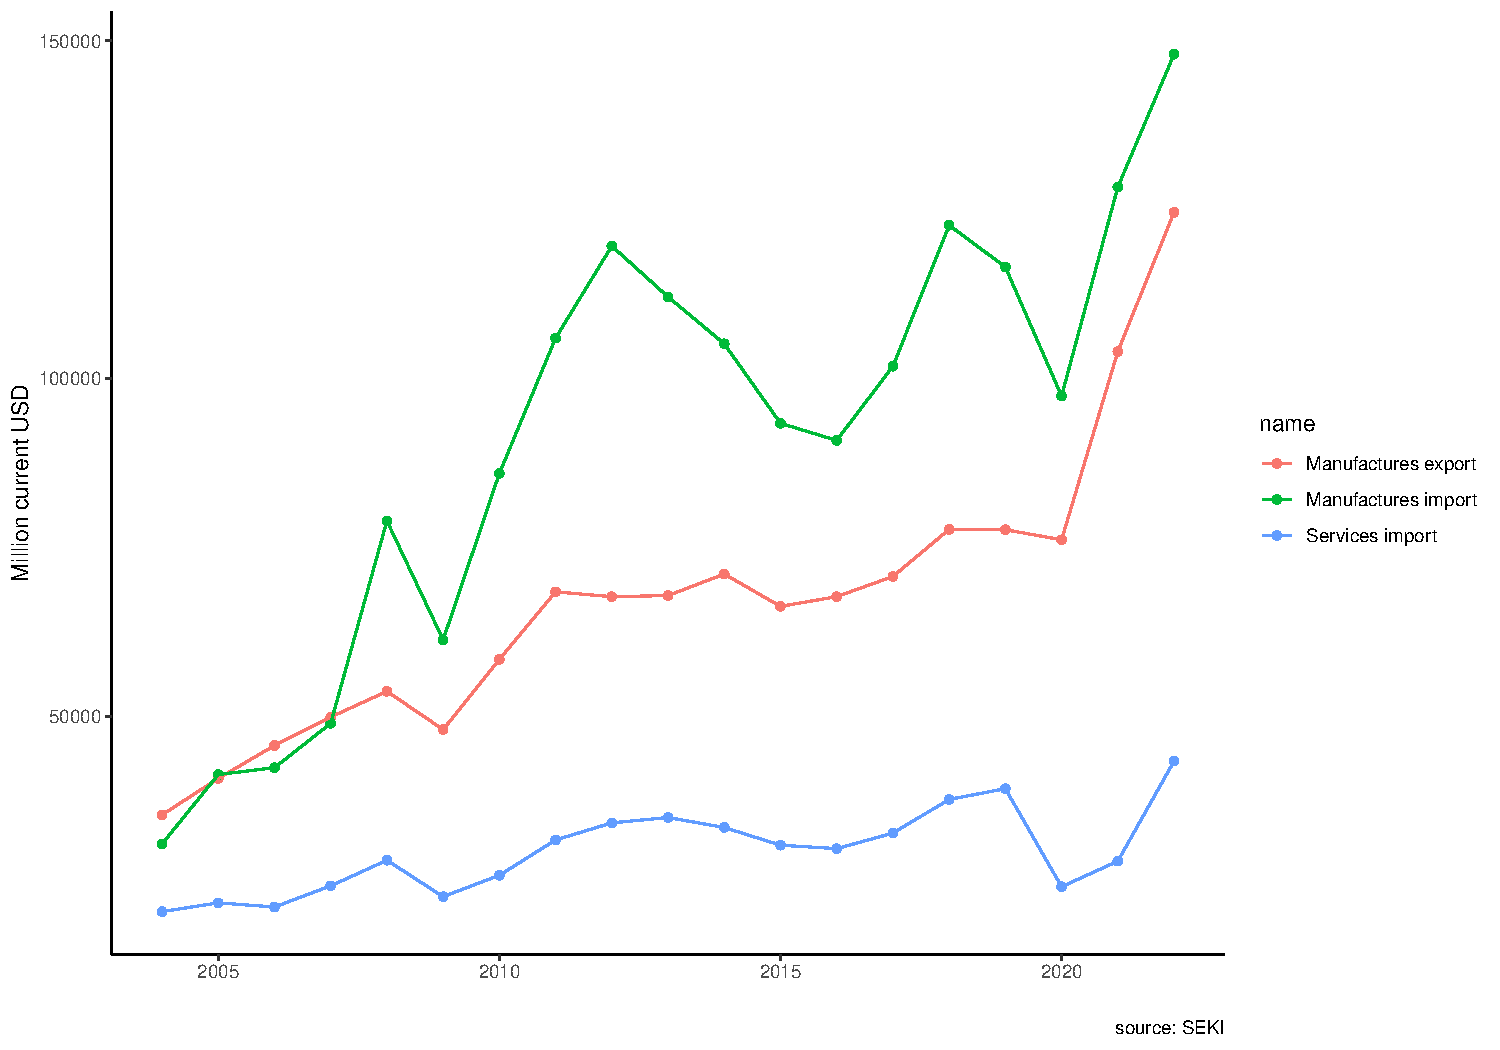
\includegraphics{Eria_services_Slides_files/figure-beamer/fig-idn-1.pdf}

}

\caption{\label{fig-idn}Indonesian trade dynamics}

\end{figure}%
\end{frame}

\begin{frame}{ARDL}
\phantomsection\label{ardl-2}
\begin{longtable}[]{@{}
  >{\raggedright\arraybackslash}p{(\columnwidth - 8\tabcolsep) * \real{0.3333}}
  >{\raggedright\arraybackslash}p{(\columnwidth - 8\tabcolsep) * \real{0.0972}}
  >{\raggedright\arraybackslash}p{(\columnwidth - 8\tabcolsep) * \real{0.1250}}
  >{\raggedright\arraybackslash}p{(\columnwidth - 8\tabcolsep) * \real{0.0972}}
  >{\raggedright\arraybackslash}p{(\columnwidth - 8\tabcolsep) * \real{0.1667}}@{}}

\caption{\label{tbl-sum2}Summary statistics}

\tabularnewline

\toprule\noalign{}
\begin{minipage}[b]{\linewidth}\raggedright
\end{minipage} & \begin{minipage}[b]{\linewidth}\raggedright
Mean
\end{minipage} & \begin{minipage}[b]{\linewidth}\raggedright
Median
\end{minipage} & \begin{minipage}[b]{\linewidth}\raggedright
SD
\end{minipage} & \begin{minipage}[b]{\linewidth}\raggedright
Histogram
\end{minipage} \\
\midrule\noalign{}
\endhead
\bottomrule\noalign{}
\endlastfoot
log value added & 7.62 & 7.67 & 1.26 & ▁▁▃▅▇▆▃▁ \\
log output & 9.01 & 9.06 & 1.21 & ▁▂▄▆▇▄▂ \\
log foreign services & 5.98 & 6.00 & 1.21 & ▂▄▇▇▄▁ \\
log domestic services & 7.23 & 7.23 & 1.25 & ▁▁▃▅▇▆▄▂▁ \\

\end{longtable}
\end{frame}

\begin{frame}{ARDL}
\phantomsection\label{ardl-3}
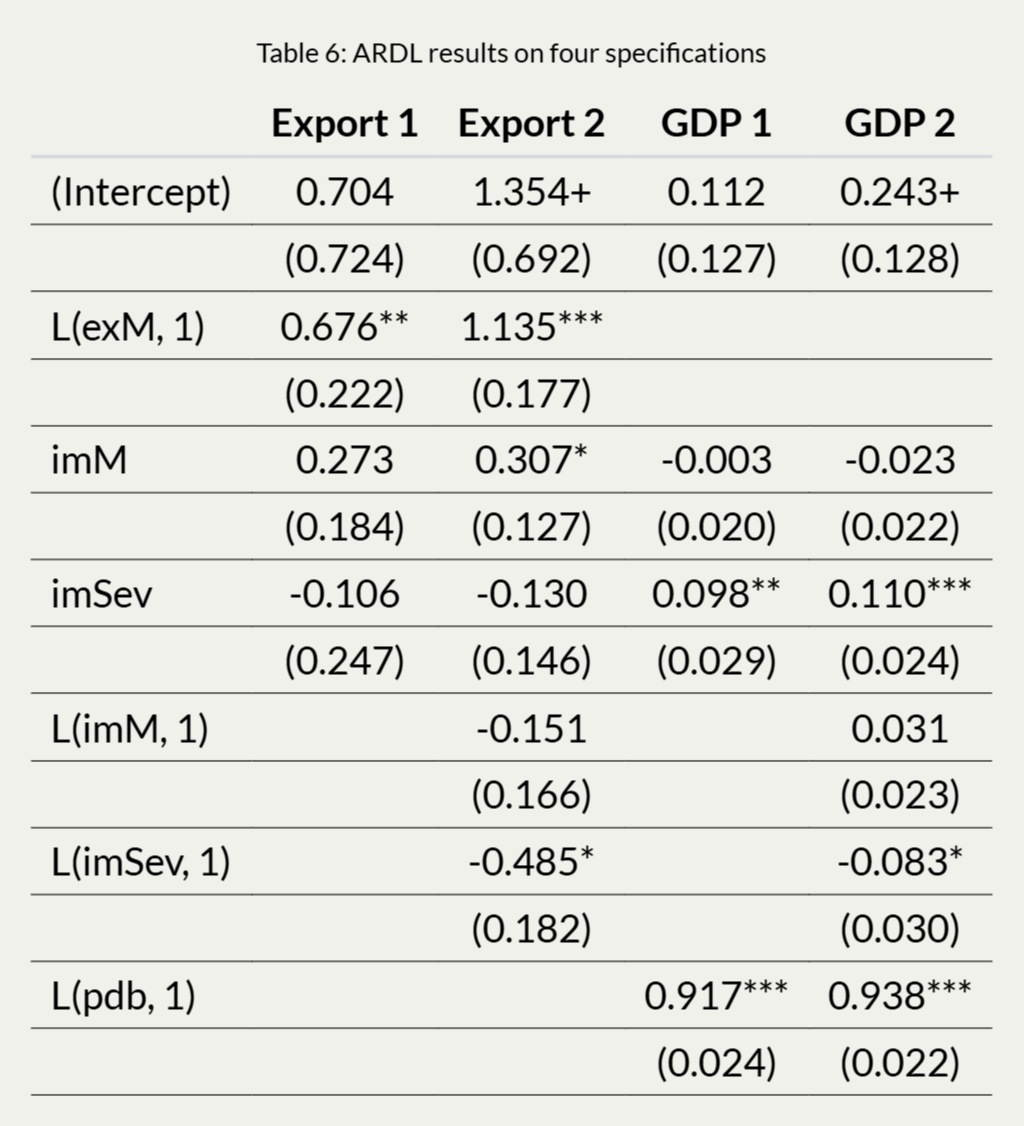
\includegraphics{plot/slides/ardl_services.png}
\end{frame}

\begin{frame}{ARDL}
\phantomsection\label{ardl-4}
\begin{itemize}
\item
  Indonesia's current import service does not seem to contribute much to
  the country's manufacturing export.
\item
  This corroborates findings in ICIO regression.
\item
  Indonesian firms does not seem to have much in house services to begin
  with, and those who do are only a small fraction of very productive
  firms (Hing and Thangavelu 2023).
\end{itemize}
\end{frame}

\begin{frame}{All in all}
\phantomsection\label{all-in-all-1}
\begin{itemize}
\item
  By itself, Indonesian services export relies on travel. Looks to be
  net-importing for some time.
\item
  Services content in manufacturing seems to be an untapped potential:
  increasing services content may be beneficial for Indonesian
  manufacturing thus the feedback mechanism a la Kimura (2018).
\item
  Exports will be needed if manufacturing to increase its services
  content beyond transport to justify the cost.
\end{itemize}
\end{frame}

\begin{frame}{Conclusion}
\phantomsection\label{conclusion}
\begin{itemize}
\item
  This chapter arguably met its goal in discussing Indonesia's service
  trade.
\item
  while ICIO is not the best, it remains the best data to look at
  services content in manufacturing (and services too, in fact i.e., the
  leap-frog)
\item
  We may need to fine-tune the discussion, so feedback is welcomed!
\end{itemize}
\end{frame}

\begin{frame}[s]{References}
\phantomsection\label{references}
\phantomsection\label{refs}
\begin{CSLReferences}{1}{0}
\bibitem[\citeproctext]{ref-baldwin}
Baldwin, Richard. 2016. \emph{The Great Convergence: Information
Technology and the New Globalization}. Book. Belknap Press of Harvard
University Press.

\bibitem[\citeproctext]{ref-baldwin2}
Baldwin, Richard, Rebecca Freeman, and Angelos Theodorakopoulos. 2024.
{``Deconstructing Deglobalization: The Future of Trade Is in
Intermediate Services.''} Journal Article. \emph{Asian Economic Policy
Review} 19 (1): 18--37.
https://doi.org/\url{https://doi.org/10.1111/aepr.12440}.

\bibitem[\citeproctext]{ref-seki}
Bank Indonesia. n.d. {``Statistik Ekonomi Dan Keuangan Indonesia.''}
Dataset. Bank Indonesia,.
\url{https://www.bi.go.id/id/statistik/ekonomi-keuangan/seki/Default.aspx\#headingFour}.

\bibitem[\citeproctext]{ref-hing}
Hing, Vutha, and Shandre Mugan Thangavelu. 2023. {``Does Servicification
Enhance Firm Productivity? Evidence from Indonesia.''} Journal Article.
\emph{Journal of Southeast Asian Economies} 40 (3): 299--317.
\url{https://remote-lib.ui.ac.id:2065/stable/27278631}.

\bibitem[\citeproctext]{ref-kimura1}
Kimura, Fukunari. 2018. {``Unbundling Regimes and Development Strategies
in ASEAN: Old Issues and New Challenges.''} Journal Article.
\emph{Southeast Asian Economies} 35 (1): 13--21.
\url{https://doi.org/10.1355/ae35-1c}.

\bibitem[\citeproctext]{ref-ebops}
Liberatore, Antonella, Rodolfo Ostolaza, Malik Bani Hani, Silvia Amiel,
Maria Fernanda L'Hopital, Markie Muryawan, Vysaul Nyirongo, and Habibur
Khan. 2021. {``C.6 Trade in Services Classifications.''} Report.
International Monetary Fund.
\url{https://www.imf.org/external/pubs/ft/bop/2021/pdf/VM2/21-05.pdf}.

\bibitem[\citeproctext]{ref-batis2}
Liberatore, Antonella, and Steen Wettstein. 2021. {``The OECD-WTO
Balanced Trade in Services Database (BaTIS).''} Report. OECD/WTO.
\url{https://www.oecd.org/content/dam/oecd/en/data/methods/OECD-WTO-Balanced-Trade-in-Services-database-methodology-BPM6.pdf}.

\bibitem[\citeproctext]{ref-lodefalk}
Lodefalk, Magnus. 2014. {``The Role of Services for Manufacturing Firm
Exports.''} Journal Article. \emph{Review of World Economics /
Weltwirtschaftliches Archiv} 150 (1): 59--82.
\url{http://remote-lib.ui.ac.id:2063/stable/44211761}.

\bibitem[\citeproctext]{ref-magiera}
Magiera, Stephen. 2011. {``Indonesia's Investment Negative List: An
Evaluation for Selected Services Sectors.''} Journal Article.
\emph{Bulletin of Indonesian Economic Studies} 47 (2): 195--219.

\bibitem[\citeproctext]{ref-melitz}
Melitz, Marc J. 2003. {``The Impact of Trade on Intra-Industry
Reallocations and Aggregate Industry Productivity.''} Journal Article.
\emph{Econometrica} 71 (6): 1695--725.
\url{https://doi.org/10.1111/1468-0262.00467}.

\bibitem[\citeproctext]{ref-ardl}
Natsiopoulos, Kleanthis, and TNickolaos G Tzeremes. 2022. {``ARDL Bounds
Test for Countegration: Replicating the Pesaran Et Al. (2001) Results
for the UK Earnings Equation Using r.''} Journal Article. \emph{Journal
of Applied Econometrics} 37 (5): 22.
\url{https://doi.org/doi.org/10.1002/jae.2919}.

\bibitem[\citeproctext]{ref-icio}
OECD. 2023. {``OECD Inter-Country Input-Output Database.''} Dataset.
\url{http://oe.cd/icio}.

\bibitem[\citeproctext]{ref-pesaran}
Pesaran, M. Hashem, and Ron Smith. 1995. {``Estimating Long-Run
Relationships from Dynamic Heterogeneous Panels.''} Journal Article.
\emph{Journal of Econometrics} 68 (1): 79--113.
https://doi.org/\url{https://doi.org/10.1016/0304-4076(94)01644-F}.

\bibitem[\citeproctext]{ref-krisna}
Syahputri, Evanti Andriani, and Krisna Gupta. 2024. {``Analysis of the
Effect of Indonesia-Japan Economic Partnership Agreement (IJEPA) on the
Trade in Service Sector in Indonesia.''} Journal Article. \emph{Jurnal
Manajemen Industri Dan Logistik} 8 (1).
\url{https://doi.org/10.30988/jmil.v8i1.1356}.

\end{CSLReferences}
\end{frame}



\end{document}
